\subsection{内自同构}

设 \(G\) 为一个群。\(\operatorname{Aut}(G)\) （群 \(G\) 的自同构所成的集合）是 \(\mathfrak{S}_{\mathbb{G}}\) 的一个子群（§ 4，第 1 号，例 2）。

命题 3. 设 G 为一个群。对 G 的每个元素 x，映射 \(\operatorname{Int}(x): y \mapsto xyx^{-1}\) 是 G 到自身的一个自同构。映射 \(\operatorname{Int}: x \mapsto \operatorname{Int}(x)\) 是 G 到 \(\operatorname{Aut}(G)\) 的群同态，其核为 G 的中心，其像为 \(\operatorname{Aut}(G)\) 的一个正规子群。

若 x、y 和 z 是 G 的元素，则 \((xyx^{-1})(xzx^{-1}) = xyzx^{-1}\) ，因此 \(\operatorname{Int}(x)\) 是 G 的一个自同态。对于 G 的元素 x 和 y，

\[
\operatorname{Int} (x) \circ \operatorname{Int} (y) = \operatorname{Int} (x y):
\]

对所有 \(z \in G\) ，有 \(x(yzy^{-1})x^{-1} = (xy)z(xy)^{-1}\) 。另一方面， \(\operatorname{Int}(e)\) 是 G 的恒等映射。因此映射 Int 是从 G 到群 G 的自同态幺半群 \(\operatorname{End}(G)\) 的幺半群同态。由于 G 的元素都可逆，映射 Int 取值于 \(\operatorname{Aut}(G)\) ，即 \(\operatorname{End}(G)\) 的可逆元素所成的集合（§ 2，第 3 号）。现在， \(xyx^{-1} = y\) 当且仅当 x 与 y 可交换，因此 \(\operatorname{Int}(x)\) 是 G 的恒等映射当且仅当 x 是中心元素。最后，设 \(\alpha\) 为 G 的一个自同构，并设 \(x \in G\) ；于是

\[
\operatorname{Int} (\alpha (x)) = \alpha \circ \operatorname{Int} (x) \circ \alpha^ {- 1}.\tag{2}
\]

对于 \(y \in G\) ,

\[
\alpha (x). y. \alpha (x) ^ {- 1} = \alpha (x). \alpha (\alpha^ {- 1} (y)). \alpha (x) ^ {- 1} = \alpha (x. \alpha^ {- 1} (y). x ^ {- 1}).
\]

因此 \(\alpha\) . Int(G) . \(\alpha^{-1} \subset \operatorname{Int}(G)\) 。

定义 4. 设 G 为一个群，\(x \in \mathbf{G}\) 。自同构 \(y \mapsto xyx^{-1}\) 称为由 \(x\) 定义的 G 的内自同构，记作 Int \(x\) 。

对于 \(x, y \in G\) ，我们也记 \(x^y = y^{-1}xy = (\operatorname{Int} y^{-1})(x)\) 。

G 的一个子群是正规的，当且仅当它在 G 的所有内自同构下稳定（§ 4，第 4 号，定义 5）。G 的一个子群若在 G 的所有自同构下稳定，则称为特征子群。群 G 的中心是一个特征子群（公式 (2)）。

群 G 的中心未必在 G 的所有自同态下稳定（习题 22）。特别地，带算子群的中心未必是稳定子群。

命题 4. 设 G 为一个群，H 为 G 的特征（相应地，正规）子群，K 为 H 的特征子群。则 K 是 G 的特征（相应地，正规）子群。

G 的自同构（相应地，内自同构）在 H 上的限制是 H 的自同构，从而保持 K 不变。

设 G 为一个群，A ⊂ G，且 \(b \in G\) 。若 \(bAb^{-1} = A\) ，则称 b 正规化 A；若对所有 \(a \in A\) 都有 \(bab^{-1} = a\) ，则称 b 中心化 A。设 A 和 B 是 G 的子集；若 B 的每个元素都正规化（相应地，中心化）A，则称 B 正规化（相应地，中心化）A。

G 中正规化（相应地，中心化）A 的 \(g \in G\) 所成的集合称为 A 的正规化子（相应地，中心化子）（参见 §1，第 5 号，定义 9）；它常记为 \(N_{G}(A)\) 或简记为 \(N(A)\) （相应地，\(C_{G}(A)\) 或 \(C(A)\) ）。它是 G 的一个子群。当 A 是 G 的子群时，\(N_{G}(A)\) 可刻画为 G 中包含 A 且使 A 在其中为正规子群的最大子群。

注记。(1) 当 G 通过内自同构作用于自身时，A 的正规化子（相应地，中心化子）就是 A 的严格稳定化子（相应地，固定子）。特别地，中心化子是正规化子的正规子群。

\begin{enumerate}
\def\labelenumi{(\arabic{enumi})}
\setcounter{enumi}{1}
\tightlist
\item
  \(b \in \mathbf{G}\) 中使 \(b\mathbf{A}b^{-1} \subset \mathbf{A}\) 的元素所成的集合是 \(\mathbf{G}\) 的一个子幺半群，即使 \(\mathbf{A}\) 是 \(\mathbf{G}\) 的子群，它也不一定是 \(\mathbf{G}\) 的子群（习题 27）。
\end{enumerate}

\subsection{轨道}

定义 5. 设 G 是一个群，E 是一个 G-集，且 \(x \in G\) 。元素 \(y \in E\) 称为在 G 的作用下与 x 共轭，如果存在元素 \(\alpha \in G\) 使得 \(y = \alpha x\) 。x 的共轭元素所成的集合称为 x 在 E 中的轨道。

关系 “y 与 x 共轭” 是一个等价关系。因为 x = ex；若 \(y = \alpha x\) ，则 \(x = \alpha^{-1} y\) ；若 \(y = \alpha x\) 且 \(z = \beta y\) ，则 \(z = \beta \alpha x\) 。轨道是此关系下的等价类。

E 的子集 X 是稳定的，当且仅当它关于共轭关系是饱和的。

G 到 E 的映射 \(\alpha\mapsto\alpha x\) 有时称为由 x 定义的轨道映射。它是 G（其中 G 通过左平移作用于自身）到 E 的一个 G-态射。G 在该映射下的像 G.x 就是 x 的轨道。

称 G 在 E 上自由地作用，如果对所有 \(x \in E\) ，由 x 定义的轨道映射都是单射，或者 G × E 到 E × E 的映射 \((g, x) \mapsto (gx, x)\) 是单射。

例子。(1) 设 G 是一个群，考虑 G 通过内自同构作用于自身。G 的两个元素若在此作用下共轭，则称为在内自同构下共轭，或简称共轭。轨道称为共轭类。类似地，G 的两个子集 H 与 \(H'\) 称为共轭的，如果存在元素 \(\alpha \in G\) 使得 \(H' = \alpha \cdot H \cdot \alpha^{-1}\) ，即它们在 G 通过内自同构作用于自身的这一作用到 \(\mathfrak{P}(G)\) 上的扩张下共轭。

\begin{enumerate}
\def\labelenumi{(\arabic{enumi})}
\setcounter{enumi}{1}
\tightlist
\item
  *在空间 \(\mathbf{R}^n\) 中，点 \(x\) 在正交群 \(\mathbf{O}(n, \mathbf{R})\) 作用下的轨道是半径为 \(\| x \|\) 的欧氏球面。*
\end{enumerate}

E 的两个共轭元素的稳定化子是 G 的共轭子群（第 2 号，命题 2）。

E 在共轭关系下的商集是 E 的轨道集合；有时记为 E/G 或 \(G\backslash E\) 。（有时记号 E/G 保留用于 E 是右 G-集的情形，而记号 \(G\backslash E\) 用于 E 是左 G-集的情形。）

设 G 是一个在集合 E 上右侧作用的群。设 H 是 G 的一个正规子群。群 G 在 E/H 上右侧作用，相应的右作用律为 \((xH, g) \mapsto xHg = xgH\) ；在此作用下，H 平凡地作用，从而得到 G/H 在 E/H 上的一个右作用。设 \(\phi\) 是 E/H 到 E/G 上的典范映射；E/G 的点在 \(\phi\) 下的原像是 G（或 G/H）在 E/H 中的轨道。因此， \(\phi\) 在取商后定义了 \((\mathrm{E}/\mathrm{H})/\mathrm{G} = (\mathrm{E}/\mathrm{H})/(\mathrm{G}/\mathrm{H})\) 到 E/G 上的一个双射，称为典范双射。

设 G（相应地，H）是在集合 E 上左作用（相应地，右作用）的群。假设 G 与 H 在 E 上的作用可交换，即

\[
(g. x). h = g. (x. h) \quad \text { for } g \in \mathrm{G}, x \in \mathrm{E} \text { and } h \in \mathrm{H}.
\]

H 在 E 上的作用也可视为 H 的反群 \(H^{0}\) 在 E 上的左作用。于是由 §4，第 9 号，命题 12 可知，把元素 \((g, h) \in G \times H^{0}\) 对应到 E 到自身的映射 \(x \mapsto g \cdot x \cdot h\) 的映射，是 \(G \times H^{0}\) 在 E 上的一个左作用。元素 \(x \in E\) 在此作用下的轨道是集合 GxH。这些轨道的集合记为 \(G\backslash E/H\) 。另一方面，G（相应地，H）的作用与关于 H（相应地，G）的作用的共轭关系相容，且轨道集合 \(G\backslash(E/H)\) （相应地，\((G\backslash E)/H\) ）等同于 \(G\backslash E/H\) ：在图中

\pandocbounded{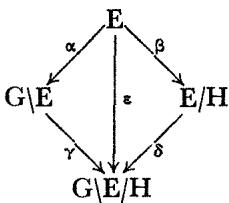
\includegraphics[keepaspectratio]{images/part001_b92675b5.jpg}}

（其中 \(\alpha, \beta, \gamma, \delta, \varepsilon\) 表示取商的典范映射）， \(\gamma \circ \alpha = \delta \circ \beta = \varepsilon\) 。

设 G 为一个群，H 为 G 的子群。考虑 H 通过右平移在 G 上的右作用（第 1 号，例 2）。轨道集合 G/H 是模 H 的左陪集集合；注意 G 依法则 \((g, xH) \mapsto gxH\) 在 G/H 上左作用（参见第 5 号）。类似地，模 H 的右陪集集合是 H 通过左平移在 G 上左作用的轨道集合 \(H\backslash G\) 。若 K 是 G 的包含 H 的子群，且 \(\Gamma\) 是模 H 的左（相应地，右）陪集，则 \(\Gamma K\) （相应地，\(K\Gamma\) ）是模 K 的左（相应地，右）陪集。映射 \(\Gamma \mapsto \Gamma K\) （相应地，\(\Gamma \mapsto K\Gamma\) ）称为 G/H 到 G/K（相应地，\(H\backslash G\) 到 \(K\backslash G\) ）的典范映射。它是满射。

设 G 为一个群，H 和 K 为 G 的两个子群。令 H 通过左平移在 G 上左作用，K 通过右平移在 G 上右作用；这两个作用可交换，故可考虑集合 \(H\backslash G/K\) 。\(H\backslash G/K\) 的元素称为 G 模 H 与 K 的双陪集。当 K = H 时，简称模 H 的双陪集。G/H 到 \(H\backslash G/H\) 上的典范映射是双射，当且仅当 H 是 G 的正规子群。

\subsection{齐次集合}

定义 6. 设 G 为一个群。G 在集合 E 上的作用称为传递的，如果存在元素 \(x \in E\) ，其轨道为 E。若 G 在 E 上的作用是传递的，则称 G-集 E 为齐次的。

也称 G 在 E 上传递地作用；或者说 E 是 G 下的齐次集。这等价于说 E 非空，且对 E 的任意元素 x 和 y，存在元素 \(\alpha \in G\) 使得 \(\alpha.x = y\) 。

例。若 E 是一个 G-集，则 E 的每个轨道（带诱导作用）都是 G 下的齐次集。

设 G 是一个群，H 是 G 的一个子群。考虑模 H 的左陪集集合 G/H。群 G 依法则 \((g, xH) \mapsto gxH\) 在 G/H 上左作用。设 N 为 H 的正规化子。群 N 依法则 \((xH, n) \mapsto xHn = xnH\) 在 G/H 上右作用。此作用在 H 上诱导出平凡作用，从而在取商后，N/H 在 G/H 上右作用。设 \(\phi: (N/H)^{0} \to S_{G/H}\) 为与此作用对应的同态。

命题 5. 在上述记号下，G/H 是一个齐次 G-集。映射 \(\phi\) 诱导出 \((\mathrm{N} / \mathrm{H})^0\) 到 G-集 G/H 的自同构群上的同构。

元素 \(\dot{e}=H\) 在 G/H 中的轨道是 G/H，由此得第一个断言。我们现在证明第二个断言。若 \(n\in N\) 通过右平移在 G/H 上定义的是恒等映射，则 \(\dot{e}.n=\dot{e}\) ，即 H.n=H，从而 \(n\in H\) 。因此

N/H 在 G/H 上右侧忠实作用，且 \(\phi\) 是单射。G 在 G/H 上的左作用与 N/H 在 G/H 上的右作用可交换，因此 N/H 的算子给出 G/H 到自身的 G-态射；由于它们是双射，这些态射必然是 G-自同构。于是 \(\phi\) 取值于 G/H 的 G-自同构所成的群 \(\Phi\) 。我们证明 \(\phi\) 的像就是 \(\Phi\) 。设 \(f \in \Phi\) 。通过结构转移，\(f(\dot{e})\) 在 G 中的稳定化子等于 \(\dot{e}\) 的稳定化子，即等于 H。设 \(n \in G\) 使得 \(f(\dot{e}) = n\dot{e}\) 。\(n\dot{e}\) 在 G 中的稳定化子是 \(nHn^{-1}\) （第 2 号，命题 2），因此 \(nHn^{-1} = H\) ，即 \(n \in N\) 。对 G/H 的每个元素 xH，有 \(f(xH) = f(x.\dot{e}) = x.f(\dot{e}) = xnH = xHn\) ，故 f 与由 n 定义的映射一致。

注记.(1) 设 G 是一个群，H 是 G 的一个子群，且 \(\phi: \mathbf{G} \to \mathfrak{S}_{\mathbf{G}/\mathbf{H}}\) 是对应于 G 在 G/H 上作用的同态。\(\phi\) 的核是 H 的诸共轭子群的交集（第 2 号，命题 2）。它也是包含在 H 中的最大正规子群（第 3 号）。特别地，G 忠实作用于 G/H 当且仅当 H 的诸共轭子群的交集缩减为 \(\{e\}\) 。

\begin{enumerate}
\def\labelenumi{(\arabic{enumi})}
\setcounter{enumi}{1}
\tightlist
\item
  设 G 为一个群，H 与 K 为其子群，且 H 是 K 的正规子群。则 K/H 在 G-集 G/H 上右作用，且 G/H 到 G/K 的典范映射在取商后定义出 G-集同构 \((G/H)/(K/H) \rightarrow G/K\) （参见第 4 号）。
\end{enumerate}

命题 6. 设 G 是一个群，E 是一个齐次 G-集， \(a \in E\) ，H 是 \(a\) 的稳定化子，且 K 是 G 中包含于 H 的子群。存在唯一的 G-态射 \(f\) ：G/K 到 E，使得 \(f(e.K) = a\) 。若 K = H，则 \(f\) 是同构。

若 \(f\) 是一个解，则 \(f(x, \mathbf{K}) = x.a\) 对所有 \(x\) 属于 \(\mathbf{G}\) 者成立，由此得唯一性；我们证明存在性。由 \(a\) 定义的轨道映射与等价关系 \(y \in x\mathbf{K}\) 在 \(\mathbf{G}\) 上相容。因为，若 \(y = xk, k \in \mathbf{K}\) ，则

\[
y. a = x k. a = x. a.
\]

映射 \(f\) 便这样由 \(G / K\) 导出到 \(H\) ，它满足 \(f(x, \mathbf{K}) = x.a\) 对所有 \(x\) 属于 \(G\) 成立。此映射是一个 G-态射，且 \(f(\mathbf{K}) = a\) 。此映射是满射的，因为它的像是 \(E\) 的一个非空稳定子集。现在设 \(K = H\) ，我们证明 \(f\) 是单射。若 \(f(x, \mathbf{H}) = f(y, \mathbf{H})\) ，则 \(x.a = y.a\) ，从而 \(x^{-1}y.a = a\) ，即 \(x^{-1}y \in H\) ，于是 \(x.H = y.H\) 。

定理 1. 设 G 是一个群。

\begin{enumerate}
\def\labelenumi{(\alph{enumi})}
\item
  每个齐次 G-集都同构于形如 G/H 的齐次 G-集，其中 H 是 G 的一个子群。
\item
  设 H 和 H' 是 G 的两个子群。G-集 G/H 与 G/H' 同构当且仅当 H 与 H' 共轭。
\end{enumerate}

由于齐次 G-集非空，断言 (a) 由命题 6 得出。我们证明 (b)。设 \(f: \mathrm{G} / \mathrm{H} \to \mathrm{G} / \mathrm{H}'\) 是一个 G-集同构。子群 H 是 H 的稳定化子，因此通过结构转移，它是 G/H' 中某元素的稳定化子。于是子群 H 与 H' 共轭（第 2 号，命题 2）。若 H' = αHα⁻¹，则 H' 是元素 α. H 在 G/H 中的稳定化子（第 2 号，命题 2），因此 G/H' 同构于 G/H（命题 6）。

例子。(1) 设 E 是一个非空集合。群 \(S_{E}\) 在 E 上传递地作用。若 x 和 y 是 E 的两个元素，则映射 \(\tau: E \to E\) （ \(\tau(x) = y\) , \(\tau(y) = x\) ，且 \(\tau(z) = z\) 对 \(z \neq x\) , y 成立）是 E 的一个置换。设 \(a \in E\) 。a 的稳定化子等同于 \(S_{F}\) ，其中 \(F = E - \{a\}\) 。于是齐次 G-集 E 同构于 \(S_{E}/S_{F}\) 。

\begin{enumerate}
\def\labelenumi{(\arabic{enumi})}
\setcounter{enumi}{1}
\tightlist
\item
  设 \(\mathbf{E}\) 是含 \(n\) 个元素的集合，\((p_i)_{i\in \mathbf{I}}\) 是整数 \(>0\) 的有限族，使得 \(\sum_{i}p_{i} = n\) 。设 \(\mathbf{X}\) 是形如 \((\mathrm{F}_i)_{i\in \mathbf{I}}\) 的 \(\mathbf{E}\) 的分拆中满足 \(\operatorname {Card}(\mathrm{F}_i) = p_i\) （对所有 \(i\) ）者所成的集合。群 \(\mathfrak{S}_{\mathbf{E}}\) 在 \(\mathbf{X}\) 上传递地作用。元素 \((\mathrm{F}_i)_{i\in \mathbf{I}}\) （属于 \(\mathbf{X}\) ）的稳定化子 H 典范同构于 \(\prod_{i\in \mathbf{I}}\mathfrak{S}_{\mathbf{F}_i}\) ，从而其阶为 \(\prod_{i\in \mathbf{I}}p_i!\) 。应用定理 1 与 §4，第 4 号，命题 4 的推论，可得到下述事实的一个新证明：
\end{enumerate}

\[
\operatorname{Card} (\mathbf {X}) = \frac {n !}{\prod_ {i \in I} p _ {i} !}.
\]

特别地，取 \(\mathbf{I} = \{1,2,\dots,r\}\) , \(\mathbf{E} = \{1,2,\dots,n\}\) ,

\[
\mathrm{F} _ {i} = \left\{p _ {1} + \dots + p _ {i - 1} + 1, \dots , p _ {1} + \dots + p _ {i} \right\}
\]

对 \(1 \leqslant i \leqslant r\) ，设 \(S\) 为 \(\tau \in \mathfrak{S}_{E}\) 中使 \(\tau|_{F_i}\) 对 \(1 \leqslant i \leqslant r\) 递增者所成的集合。若 \((G_1, \ldots, G_r) \in X\) ，则存在唯一的 \(\tau \in S\) 把 \((F_1, \ldots, F_r)\) 映为 \((G_1, \ldots, G_r)\) 。换言之，\(\mathfrak{S}_{E}\) 模 \(H\) 的每个左陪集与 \(S\) 恰好交于一点。

\begin{enumerate}
\def\labelenumi{(\arabic{enumi})}
\setcounter{enumi}{2}
\tightlist
\item
  *设 \(n\) 为整数 \(\geqslant 1\) 。正交群 \(\mathbf{O}(n, \mathbf{R})\) 在 \(\mathbf{S}_{n-1}\) （ \(\mathbf{R}^n\) 中的单位球面）上传递地作用。点 \((0, \ldots, 0, 1)\) 的稳定化子等同于正交群 \(\mathbf{O}(n-1, \mathbf{R})\) 。于是齐次 \(\mathbf{O}(n, \mathbf{R})\) -集 \(\mathbf{S}_{n-1}\) 同构于 \(\mathbf{O}(n, \mathbf{R}) / \mathbf{O}(n-1, \mathbf{R})\) 。*
\end{enumerate}

\subsection{齐次主集}

定义 7. 设 G 为一个群。G 在集合 E 上的一个作用称为单传递的，如果存在 E 中的一个元素 x，使得由 x 定义的轨道映射是双射。集合 E 连同 G 在 E 上的一个单传递左作用，称为 G 下的左齐次主 G-集（或 G 下的左齐次主集）。

这等同于说 G 在 E 上自由且传递地作用，或者也说存在一个元素 \(x \in E\) 使得由 x 定义的轨道映射是 G-集 G（其中 G 通过左平移作用）到 E 的一个同构；或者等价地，满足以下两个条件：

\begin{enumerate}
\def\labelenumi{(\roman{enumi})}
\item
  E 是非空的。
\item
  对于所有元素 \(x\) 和 \(y\) 于 \(\mathbf{E}\) ，存在且仅存在一个元素 \(\alpha \in \mathbf{G}\) 的集合，使得 \(\alpha x = y\) .
\end{enumerate}

条件(ii)也等价于以下条件：

\begin{enumerate}
\def\labelenumi{(\roman{enumi})}
\setcounter{enumi}{2}
\tightlist
\item
  映射 \((\alpha, x) \mapsto (\alpha x, x)\) 是从 \(G \times E\) 到 \(E \times E\) .
\end{enumerate}

我们将定义右齐次主 G-集的任务留给读者。

例子。(1) 设 G 通过左（相应地，右）平移作用于自身。这样便在 G 上定义了一个左（相应地，右）齐次主 G-集结构，它有时记为 \(G_{s}\) （相应地，\(G_{d}\) ）。

\begin{enumerate}
\def\labelenumi{(\arabic{enumi})}
\setcounter{enumi}{1}
\item
  设 E 是交换群 G 下的齐次集。若 G 忠实作用于 E，则后者是齐次主 G-集。
\item
  设 E 和 F 是两个同构的、带同一种类结构的集合，令 \(\operatorname{Isom}(\mathbf{E}, \mathbf{F})\) 为 E 到 F 上（带给定结构的）同构所成的集合。E 的（带给定结构的）自同构群 \(\operatorname{Aut}(\mathbf{E})\) 在 \(\operatorname{Isom}(\mathbf{E}, \mathbf{F})\) 上依法则 \((\sigma, f) \mapsto f \circ \sigma\) 右作用，且 \(\operatorname{Isom}(\mathbf{E}, \mathbf{F})\) 是一个右齐次主 \(\operatorname{Aut}(\mathbf{E})\) -集。类似地，群 \(\operatorname{Aut}(\mathbf{F})\) 在 \(\operatorname{Isom}(\mathbf{E}, \mathbf{F})\) 上依法则 \((\sigma, f) \mapsto \sigma \circ f\) 左作用，且 \(\operatorname{Isom}(\mathbf{E}, \mathbf{F})\) 是一个左齐次主 \(\operatorname{Aut}(\mathbf{F})\) -集。
\item
  *向量空间的加法群下的齐次主集称为仿射空间（参见 II，§ 9，第 1 号）。*
\end{enumerate}

齐次主 G-集 \(G_{s}\) （例 1）的自同构群是 G 的右平移群，它等同于 \(G^{0}\) （第 5 号，命题 5）。设 E 是一个齐次主 G-集，a 是 E 的一个元素。由 a 定义的轨道映射 \(\omega_{a}\) 是 G-集 \(G_{s}\) 到 E 上的同构。通过结构转移，得到一个同构 \(\psi_{a}\) ，它把 \(G^{0}\) 映到 Aut(E) 上。应当注意， \(\psi_{a}\) 一般依赖于 a；更确切地说，对于 \(\alpha \in G\) ，

\[
\psi_ {\alpha a} = \psi_ {a} \circ \operatorname{Int} _ {\mathbf {G} ^ {0}} (\alpha) = \psi_ {a} \circ \operatorname{Int} (\alpha^ {- 1}).\tag{3}
\]

因为，用 \(\delta_{a}\) 表示 G 上的平移 \(x\mapsto x\alpha\) ，

\[
\omega_ {\alpha a} = \omega_ {a} \circ \delta_ {\alpha}
\]

和

\[
\psi_ {a} (x) = \omega_ {a} \circ \delta_ {x} \circ \omega_ {a} ^ {- 1}, \quad x \in G,
\]

因此

\[
\psi_ {\alpha a} (x) = \omega_ {a} \circ \delta_ {\alpha} \circ \delta_ {x} \circ \delta_ {\alpha} ^ {- 1} \circ \omega_ {a} ^ {- 1} = \omega_ {a} \circ \delta_ {\alpha^ {- 1} x \alpha} \circ \omega_ {a} ^ {- 1} = \psi_ {a} (\alpha^ {- 1} x \alpha).
\]

\subsection{有限集合的置换群}

若 E 是含 n 个元素的有限集，则对称群 \(S_{E}\) （§ 4，第 1 号）是阶为 \(n!\) 的有限群。当 E 是自然数集 N 的区间 \([1, n]\) 时，相应的对称群记为 \(S_{n}\) ；任何含 n 个元素的集合的对称群都同构于 \(S_{n}\) 。

定义 8. 设 E 为有限集， \(\zeta \in \mathfrak{S}_{\mathrm{E}}\) 为 E 的一个置换， \(\bar{\zeta}\) 为 \(\mathfrak{S}_{\mathrm{E}}\) 中由 \(\zeta\) 生成的子群。\(\zeta\) 称为轮换，如果在 \(\bar{\zeta}\) 于 E 的作用下恰存在一条不缩减为单个元素的轨道。这条轨道称为 \(\zeta\) 的支集。

设 \(\zeta\) 为一个轮换。支集 \(\operatorname{supp}(\zeta)\) （即 \(\zeta\) 的支集）是由 \(x \in E\) 中满足 \(\zeta(x) \neq x\) 的元素组成的集合。

轮换 \(\zeta\) 的阶等于其支集的基数。子群 \(\bar{\zeta}\) 由 \(\zeta\) 生成，它在 \(\operatorname{supp}(\zeta)\) 上传递且忠实地作用。由于 \(\zeta\) 是交换的， \(\operatorname{supp}(\zeta)\) 是 \(\bar{\zeta}\) 下的一个主集（第 6 号，例 2），因此 \(\operatorname{Card}(\operatorname{supp}(\zeta)) = \operatorname{Card}(\bar{\zeta})\) 。

引理 1. 设 \((\zeta_{i})_{i\in I}\) 是一族支集两两不相交的轮换。则诸 \(\zeta_{i}\) 两两可交换。设 \(\sigma = \prod_{i\in I}\zeta_{i}\) ， \(\overline{\sigma}\) 为由 \(\sigma\) 生成的子群。则 \(\sigma(x) = \zeta_{i}(x)\) 对 \(x\in S_{i}, i\in I\) 成立，而 \(\sigma(x) = x\) 对 \(x\notin \bigcup_{i\in I}S_{i}\) 成立。映射 \(i\mapsto S_i\) 是 I 到不由单个元素组成的 \(\overline{\sigma}\) -轨道所成集合上的一个双射。

设 \(\zeta\) 和 \(\zeta'\) 是两个支集不相交的轮换。如果

\[
x \notin \operatorname{supp} (\zeta) \cup \operatorname{supp} \left(\zeta^ {\prime}\right),
\]

则 \(\zeta\zeta'(x) = \zeta'\zeta(x) = x\) 。若 \(x\) 属于 \(\zeta\) 的支集，则 \(\zeta'(x) = x\) 且 \(\zeta(x)\) 属于 \(\zeta\) 的支集，因此 \(\zeta\zeta'(x) = \zeta'\zeta(x) = \zeta(x)\) 。类似地，当 \(x\) 属于 \(\zeta'\) 的支集时， \(\zeta'\zeta(x) = \zeta\zeta'(x) = \zeta'(x)\) 。因此 \(\zeta\zeta' = \zeta'\zeta\) 。于是诸 \(\zeta_i\) 两两可交换，且对于 \(i \in I\) 和 \(x \in S_i\) , \(\sigma(x) = \zeta_i(x) \in S_i\) 。映射 \(\sigma\) 与 \(\zeta_i\) 在 \(S_i\) 上重合，故 \(S_i\) 在 \(\sigma\) 下稳定，且 \(\mathfrak{S}_{S_i}\) 中由 \(\sigma\) 在 \(S_i\) 上的限制所生成的子群在 \(S_i\) 上传递地作用；因此 \(S_i\) 是一条 \(\overline{\sigma}\) -轨道。由于诸 \(S_i\) 非空且两两不相交，映射 \(i \mapsto S_i\) 是单射。由于 \(\bigcup_{i} S_i\) 是 \(x\) 满足 \(\sigma(x) \neq x\) 的那些元素组成的集合，每条不由单个元素组成的 \(\overline{\sigma}\) -轨道都是某个 \(S_i\) 。

命题 7. 设 E 是一个有限集，且 \(\sigma\) 是 E 的一个置换。存在唯一的由轮换组成的有限集 C，满足以下两个条件：

\begin{enumerate}
\def\labelenumi{(\alph{enumi})}
\item
  C 中元素的支集两两不相交；
\item
  \(\sigma = \prod_{\zeta \in C} \zeta\) （由引理 1 ， \(C\) 的元素两两可交换）。设 \(\bar{\sigma}\) 为由 \(\sigma\) 生成的子群， \(S\) 为不由单个元素组成的 \(\bar{\sigma}\) -轨道所成的集合。对 \(s \in S\) ，令 \(\zeta_s(x) = \sigma(x)\) （若 \(x \in s\) ），并令 \(\zeta_s(x) = x\) （若 \(x \notin s\) ）。对所有 \(s \in S\) , \(\zeta_s\) 是支集为 \(s\) 的一个轮换，且 \(\sigma = \prod_{s \in S} \zeta_s\) ，这只需把两边作用于 \(E\) 的任意元素即可看出。\(C\) 的唯一性由引理 1 可得。
\end{enumerate}

定义 9. 2 阶轮换称为对换。

设 \(x\) 和 \(y\) 是 \(E\) 的两个不同元素。用 \(\tau_{x,y}\) 表示支集为 \(\{x, y\}\) 的唯一的对换。

对 E 的每个置换 \(\sigma\) ，置换 \(\sigma. \tau_{x,y}. \sigma^{-1}\) 是支集为 \(\{\sigma(x), \sigma(y)\}\) 的一个对换。因此：

\[
\sigma . \tau_ {x, y}. \sigma^ {- 1} = \tau_ {\sigma (x), \sigma (y)}.\tag{4}
\]

于是，对换在群 \(\mathfrak{S}_{\mathbb{E}}\) 中构成一个共轭类。

命题 8. 设 E 为有限集。群 \(\mathfrak{S}_{\mathrm{E}}\) 由对换生成。

对每个置换 \(\sigma\) ，令 \(F_{\sigma}\) 为由 \(x \in E\) 中满足 \(\sigma(x) = x\) 的元素组成的集合。我们对 \(p\) 作递降归纳来证明：每个置换 \(\sigma\) ，只要 \(\operatorname{Card}(F_{\sigma}) = p\) ，就是对换之积。若 \(p \geqslant \operatorname{Card}(E)\) ，则置换 \(\sigma\) 是 \(E\) 的恒等映射；它是对换的空族之积。若 \(p < \operatorname{Card}(E)\) ，设性质已对每个置换 \(\sigma'\) （ \(\operatorname{Card}(F_{\sigma'}) > p\) ）证明。现在 \(E - F_{\sigma} \neq \varnothing\) ；取 \(x \in E - F_{\sigma}\) 及 \(y \in \sigma(x)\) 。则 \(y \neq x\) 且 \(y \in E - F_{\sigma}\) 。令 \(\sigma' = \tau_{x,y} \cdot \sigma\) 。集合 \(F_{\sigma'}\) 包含 \(F_{\sigma}\) 与 \(x\) ，故 \(\operatorname{Card}(F_{\sigma'}) > \operatorname{Card}(F_{\sigma}) = p\) 。由归纳假设， \(\sigma'\) 是对换之积，从而 \(\sigma = \tau_{x,y} \cdot \sigma'\) 是对换之积。

命题 9. 设 \(n\) 为整数 \(\geqslant 0\) 。群 \(\mathfrak{S}_n\) 由诸对换 \((\tau_{i,i+1})_{1\leqslant i\leqslant n-1}\) 生成。

根据命题 8 ，只需证明每个对换 \(\tau_{p,q}\) （ \(1 \leqslant p < q \leqslant n\) ）属于由诸 \(\tau_{i,i+1}\) （ \(1 \leqslant i \leqslant n-1\) ）生成的子群 H 。我们对 \(q-p\) 作归纳来证明这一点。对 \(q-p=1\) ，这是显然的。若 \(q-p>1\) ，则（公式 (4)） \(\tau_{p,q} = \tau_{q-1,q}\tau_{p,q-1}\tau_{q-1,q}\) 。由归纳假设 \(\tau_{p,q-1} \in H\) ，从而 \(\tau_{p,q} \in H\) 。

若 \(\sigma \in \mathfrak{S}_n\) ，则每个有序对 \((i,j)\) （ \([1,n]\) 的元素，满足 \(i < j\) 且 \(\sigma(i) > \sigma(j)\) ）称为 \(\sigma\) 的一个逆序。用 \(\nu(\sigma)\) 表示 \(\sigma\) 的逆序的个数。

设 P 为从 \(Z^{n}\) 到 Z 的映射所成的加法群。对 \(f \in P\) 与 \(\sigma \in S_{n}\) ，令 \(\sigma f\) 为 P 中由下式定义的元素

\[
\sigma f (z _ {1}, \dots , z _ {n}) = f (z _ {\sigma (1)}, \dots , z _ {\sigma (n)}).\tag{5}
\]

这样定义的 \(\mathfrak{S}_n\) 在 \(\mathbf{P}\) 上的作用是一个群作用；对所有 \(\sigma, \tau \in \mathfrak{S}_n\) 和 \(f \in \mathbf{P}, ef = f\) 且

\[
\begin{array}{r l} \left(\tau (\sigma f)\right) (z _ {1}, \dots , z _ {n}) & = \sigma f (z _ {\tau (1)}, \dots , z _ {\tau (n)}) = f (z _ {\tau \sigma (1)}, \dots , z _ {\tau \sigma (n)}) \\ & = ((\tau \sigma) f) (z _ {1}, \dots , z _ {n}). \end{array}
\]

公式 (5) 表明 \(\sigma(-f) = -\sigma f\) 对 \(\sigma \in \mathfrak{S}_n\) 和 \(f \in P\) 成立。

设 \(p\) 为 P 中由下式定义的元素

\[
p (z _ {1}, \dots , z _ {n}) = \prod_ {i <   j} (z _ {j} - z _ {i}).\tag{6}
\]

引理 2. \(p \neq 0\) ，且 \(\sigma p = (-1)^{\nu(\sigma)}\) 对 \(\sigma \in \mathfrak{S}_n\) 成立。

\(p(1,2,\ldots,n) = \prod_{i < j}(j - i)\neq 0\) ，因此 \(p\neq 0\) 。另一方面，若 \(\sigma \in \mathfrak{S}_n\) ，则

\[
\sigma p (z _ {1}, \dots , z _ {n}) = p (z _ {\sigma (1)}, \dots , z _ {\sigma (n)}) = \prod_ {i <   j} (z _ {\sigma (j)} - z _ {\sigma (i)}).
\]

设 C 为有序对 \((i,j)\) 所成的集合，满足 \(1 \leqslant i \leqslant n\) , \(1 \leqslant j \leqslant n\) ， i \textless{} j 。在 C 上定义置换 \(\theta\) 如下：令 \(\theta(i,j) = (\sigma(i), \sigma(j))\) 若 \((i,j)\) 不是逆序；令 \(\theta(i,j) = (\sigma(j), \sigma(i))\) 若 \((i,j)\) 是逆序。由此可得 \(\sigma p = (-1)^{\nu(\sigma)} p\) 。

定理 2. 设 E 是一个有限集。存在唯一的同态 \(\varepsilon\) ：从 \(\mathfrak{S}_n\) 到乘法群 \(\{-1, +1\}\) ，使 \(\varepsilon(\tau) = -1\) 对每个对换 \(\tau\) 成立。

唯一性由命题 8 得出。我们证明存在性。通过结构转移，可设 \(\mathbf{E} = [1, n]\) 。采用上述记号，令 \(\varepsilon(\sigma) = (-1)^{\nu(\sigma)}\) 。则（引理 2）

\[
\sigma (\sigma^ {\prime} p) = \sigma (\varepsilon (\sigma^ {\prime}) p) = \varepsilon (\sigma^ {\prime}) (\sigma p) = \varepsilon (\sigma^ {\prime}) \varepsilon (\sigma) p.
\]

另一方面，

\[
\sigma (\sigma^ {\prime} p) = (\sigma \sigma^ {\prime}) p = \varepsilon (\sigma \sigma^ {\prime}) p.
\]

由于 \(p \neq -p\) ，由此可得 \(\varepsilon(\sigma\sigma') = \varepsilon(\sigma)\varepsilon(\sigma')\) ，故 \(\varepsilon\) 是一个同态。我们现在证明，对每个对换 \(\tau, \varepsilon(\tau) = -1\) 。\(\nu(\tau_{n-1,n}) = 1\) ，故 \(\varepsilon(\tau_{n-1,n}) = -1\) 。由于每个对换 \(\tau\) 都与 \(\tau_{n-1,n}\) 共轭，且群 \(\{-1, +1\}\) 是交换的，故 \(\varepsilon(\tau) = \varepsilon(\tau_{n-1,n}) = -1\) 。

定义 10. 在定理 2 的记号下，数 \(\varepsilon(\sigma)\) （也记作 \(\varepsilon_{\sigma}\) ）称为置换 \(\sigma\) 的符号。同态 \(\varepsilon\) 的核称为 E 的交错群。

\(\sigma\) 称为偶置换（相应地，奇置换），如果 \(\varepsilon(\sigma) = 1\) （相应地， \(\varepsilon(\sigma) = -1\) ）。E 的交错群记为 \(\mathfrak{A}_{\mathbb{E}}\) 。它是 \(\mathfrak{S}_{\mathbb{E}}\) 的一个正规子群。当 \(\mathbf{E} = [1, n]\) 时，简记为 \(\mathfrak{A}_{n}\) 。当 E 的基数 \(n\) 为 \(\geqslant 2\) 时，它是指数为 2 的子群，因此阶为 \(n! / 2\) 。可以证明，对 \(n = 3\) 或 \(n \geqslant 5\) ，群 \(\mathfrak{A}_{n}\) 是单群（参见习题 16）。

例。若 \(\sigma\) 是一个阶为 \(d\) 的轮换，则

\[
\varepsilon (\sigma) = (- 1) ^ {d - 1}.
\]

置换的逆序数

\[
(1, 2, 3, \dots , d) \mapsto (d, 1, 2, \dots , d - 1)
\]

等于 \(d - 1\) 。

\section{扩张、可解群、幂零群}

在本段中，除非另有明确说明，群运算均以乘法形式书写。

\subsection{扩张}

定义 1. 设 F 和 G 是两个群。G 被 F 的扩张是一个三元组 \(\mathcal{E} = (\mathrm{E}, i, p)\) ，其中 E 是一个群， \(i\) 是 F 到 E 内的单射同态， \(p\) 是 E 到 G 上的满射同态，使得 \(\operatorname{Im}(i) = \operatorname{Ker}(p)\) 。同态 \(s: \mathrm{G} \to \mathrm{E}\) （相应地， \(r: \mathrm{E} \to \mathrm{F}\) ），若满足 \(p \circ s = \operatorname{Id}_{\mathbf{G}}\) （相应地， \(r \circ i = \operatorname{Id}_{\mathbf{F}}\) ），则称为扩张 \(\mathcal{E}\) 的截面（相应地，收缩）。

扩张 \(\mathcal{E} = (\mathrm{E}, i, p)\) （ \(\mathbf{G}\) 被 \(\mathbf{F}\) 的扩张）常用图表 \(\mathcal{E}: \mathrm{F} \xrightarrow{i} \mathrm{E} \xrightarrow{p} \mathrm{G}\) 表示，其中 \(i\) 和 \(p\) 在不会引起混淆时有时省略。有时也简单地说群 \(\mathbf{E}\) 是 \(\mathbf{G}\) 被 \(\mathbf{F}\) 的扩张。

群 E 是 G 被 F 的扩张，当且仅当它包含一个同构于 F 的正规子群 \(F'\) ，使得商群 \(E/F'\) 同构于 G。

一个扩张 \(\mathcal{E}\colon\mathrm{F}\xrightarrow{i}\mathrm{E}\xrightarrow{p}\mathrm{G}\) 称为中心扩张，如果像 \(i(\mathrm{F})\) 包含在 E 的中心内；这仅当 F 是交换群时才可能。

设 \(\mathcal{E}:\mathrm{F}\xrightarrow{i}\mathrm{E}\xrightarrow{p}\mathrm{G}\) 和 \(\mathcal{E}':\mathrm{F}\xrightarrow{i'}\mathrm{E}'\xrightarrow{p'}\mathrm{G}\) 是 G 被 F 的两个扩张。\(\mathcal{E}\) 到 \(\mathcal{E}'\) 的态射是一个同态 \(u:\mathrm{E}\to\mathrm{E}'\) ，满足 \(p'\circ u=p\) 与 \(u\circ i=i'\) ，或者换句话说，使得下图交换：

\pandocbounded{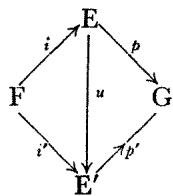
\includegraphics[keepaspectratio]{images/part001_e41623d9.jpg}}

命题 1. 设 \(\mathcal{E}: F \xrightarrow{i} E \xrightarrow{p} G\) 和 \(\mathcal{E}': F \xrightarrow{i'} E' \xrightarrow{p'} G\) 是 \(G\) 被 \(F\) 的扩张。若 \(u: E \to E'\) 是 \(\mathcal{E}\) 到 \(\mathcal{E}'\) 的态射，则 \(u\) 是 \(E\) 到 \(E'\) 上的同构，且 \(u^{-1}\) 是 \(\mathcal{E}'\) 到 \(\mathcal{E}\) 的态射。

设 \(x \in E\) 满足 \(u(x) = e\) 。则 \(p(x) = p'(u(x)) = e\) ，因此 \(x \in i(F)\) 。设 \(y \in F\) 满足 \(x = i(y)\) ；则 \(i'(y) = u(i(y)) = e\) 。由于 \(i'\) 是单射，有 \(y = e\) 与 \(x = e\) 。因此 \(u\) 是单射。根据 §4 第 6 号命题 7 的推论 1 ， \(u\) 是满射，因为 \(u(i(F)) = i'(F)\) 。最后一个断言是显然的。

换句话说，扩张 \(\mathcal{E}\) 与 \(\mathcal{E}'\) 同构，当且仅当存在 \(\mathcal{E}\) 到 \(\mathcal{E}'\) 的态射。

设 \(\mathbf{F}\) 和 \(\mathbf{G}\) 是两个群，记 \(\mathbf{E}_0 = \mathbf{F} \times \mathbf{G}\) ；令 \(i: \mathbf{F} \to \mathbf{E}_0\) 为典范单射， \(p: \mathbf{E}_0 \to \mathbf{G}\) 为典范投影。\(\mathbf{G}\) 被 \(\mathbf{F}\) 的扩张中，凡同构于扩张 \(\mathcal{E}_0: \mathbf{F} \xrightarrow{i} \mathbf{E}_0 \xrightarrow{p} \mathbf{G}\) 者，都称为平凡扩张。

命题 2. 设 \(\mathcal{E}:\mathrm{F}\xrightarrow{i}\mathrm{E}\xrightarrow{p}\mathrm{G}\) 是 \(\mathrm{G}\) 被 \(\mathrm{F}\) 的一个扩张。下列条件等价：

\begin{enumerate}
\def\labelenumi{(\roman{enumi})}
\item
  \(\mathcal{E}\) 是一个平凡扩张；
\item
  \(\mathcal{E}\) 有一个收缩 \(r\) ；
\item
  \(\mathcal{E}\) 有一个截面 \(s\) ，使得 \(s(\mathbf{G})\) 包含于 \(i(\mathbf{F})\) 的中心化子中；
\end{enumerate}

显然 (i) 蕴含 (ii) 与 (iii)。若 (ii) 成立，则映射 \((r, p): \mathbf{E} \to \mathbf{F} \times \mathbf{G}\) 是 \(\mathcal{E}\) 到 \(\mathcal{E}_0\) 的态射，由此得 (i)。若 (iii) 成立，则从 \(\mathbf{F} \times \mathbf{G}\) 到 \(\mathbf{E}\) 的、对应于 \((i, s)\) 的同态（ \(\S 4\) ，第 9 号，命题 12）是 \(\mathcal{E}_0\) 到 \(\mathcal{E}\) 的态射，由此得 (i)。

可能有这样的情形：扩张 \(\mathcal{E}:\mathbf{F}\to\mathbf{E}\to\mathbf{G}\) 并不平凡，而群 \(\mathbf{E}\) 却同构于 \(\mathbf{F}\times\mathbf{G}\) （习题 6）。

定义 2. 设 F 和 G 是两个群， \(\tau\) 是 G 到 F 的自同构群的一个同态。记 \(\tau(g)(f) = {}^g f\) （对 \(g \in G\) 与 \(f \in F\) ）。集合 \(\mathbf{F} \times \mathbf{G}\) 赋以合成律

\[
((f, g), (f ^ {\prime}, g ^ {\prime})) \mapsto (f, g) \cdot_ {\tau} (f ^ {\prime}, g ^ {\prime}) = (f. ^ {g} f ^ {\prime}, g g ^ {\prime})\tag{1}
\]

称为 G 与 F 关于 \(\tau\) 的外半直积。

G 与 F 关于 \(\tau\) 的外半直积记作 \(F \times_{\tau} G\) 。

命题 3. 外半直积 \(\mathbf{F} \times_{\tau} \mathbf{G}\) 是一个群。映射 \(i: \mathbf{F} \to \mathbf{F} \times_{\tau} \mathbf{G}\) 由 \(i(f) = (f, e)\) 定义，映射 \(p: \mathbf{F} \times_{\tau} \mathbf{G} \to \mathbf{G}\) 由 \(p(f, g) = g\) 定义，映射 \(s: \mathbf{G} \to \mathbf{F} \times_{\tau} \mathbf{G}\) 由 \(s(g) = (e, g)\) 定义，它们都是群同态。三元组 \((\mathbf{F} \times_{\tau} \mathbf{G}, i, p)\) 是 \(\mathbf{G}\) 被 \(\mathbf{F}\) 的一个扩张，而 \(s\) 是该扩张的一个截面。

我们有：

\[
\begin{array}{r l} ((f, g) \cdot_ {\tau} (f ^ {\prime}, g ^ {\prime})) \cdot_ {\tau} (f ^ {\prime \prime}, g ^ {\prime \prime}) & = (f. ^ {g} f ^ {\prime}, g g ^ {\prime}) \cdot_ {\tau} (f ^ {\prime \prime}, g ^ {\prime \prime}) \\ & = (f. ^ {g} f ^ {\prime}. ^ {g g ^ {\prime}} f ^ {\prime \prime}, g g ^ {\prime} g ^ {\prime \prime}); \\ (f, g) \cdot_ {\tau} ((f ^ {\prime}, g ^ {\prime}) \cdot_ {\tau} (f ^ {\prime \prime}, g ^ {\prime \prime})) & = (f, g) \cdot_ {\tau} (f ^ {\prime}. ^ {g ^ {\prime}} f ^ {\prime \prime}, g ^ {\prime} g ^ {\prime \prime}) \\ & = (f. ^ {g} (f ^ {\prime}. ^ {g ^ {\prime}} f ^ {\prime \prime}), g g ^ {\prime} g ^ {\prime \prime}). \end{array}
\]

现在， \({}^{g}(f'.{}^{g'}f'') = {}^{g}f'.{}^{gg'}f''\) ，这表明由 (1) 定义的合成律是结合的。元素 \((e, e)\) 是该律下的单位元。元素 \((f, g)\) 以 \((^{g^{-1}}f^{-1}, g^{-1})\) 为逆元。因此 \(F \times_{\tau} G\) 上的合成律是群律。其余断言是显然的。

采用命题 3 的记号，用 \(E_{\tau}\) 表示扩张

\[
\mathrm{F} \xrightarrow {i} \mathrm{F} \times_ {\tau} \mathrm{G} \xrightarrow {p} \mathrm{G}.
\]

设 \(\mathcal{E}'\colon F\stackrel{i'}{\to}E'\stackrel{p'}{\to}G\) 是 \(G\) 被 \(F\) 的扩张， \(s'\colon G\to E'\) 是 \(\mathcal{E}'\) 的一个截面。我们定义一个运算 \(\tau\) （ \(G\) 在群 \(F\) 上的运算）如下：

\[
i ^ {\prime} (\tau (g, f)) = s ^ {\prime} (g) i ^ {\prime} (f) s ^ {\prime} (g) ^ {- 1} = \operatorname{Int} (s ^ {\prime} (g)) (i ^ {\prime} (f)).\tag{2}
\]

命题 4. 采用上述记号，存在唯一的同构 \(u\) ，它把 \(\mathcal{E}_{\tau}\) 映到 \(\mathcal{E}'\) 上，使得 \(u \circ s = s'\) 。

\((f, g) = (f, e) \cdot_ {\tau} (e, g) = i(f).s(g)\) 。因此，如果 u 是该问题的一个解，则必然有 \(u(f,g)=i'(f).s'(g)\) ，从而 u 的唯一性成立。我们证明存在性。我们记 \(u(f,g)=i'(f).s'(g)\) 。则

\[
\begin{array}{r l} u (f, g) \cdot u (f ^ {\prime}, g ^ {\prime}) & = i ^ {\prime} (f) s ^ {\prime} (g) i ^ {\prime} (f ^ {\prime}) s ^ {\prime} (g ^ {\prime}) \\ & = i ^ {\prime} (f) (s ^ {\prime} (g) i ^ {\prime} (f ^ {\prime}) s ^ {\prime} (g) ^ {- 1}) s ^ {\prime} (g) s ^ {\prime} (g ^ {\prime}) \\ & = i ^ {\prime} (f) i ^ {\prime} (\tau (g, f ^ {\prime})) \cdot s ^ {\prime} (g) s ^ {\prime} (g ^ {\prime}) \\ & = i ^ {\prime} (f \cdot \tau (g, f ^ {\prime})) \cdot s ^ {\prime} (g g ^ {\prime}) \\ & = u ((f, g) \cdot_ {\tau} (f ^ {\prime}, g ^ {\prime})). \end{array}
\]

因此， \(u\) 是 \(\mathbf{F} \times_{\tau} \mathbf{G}\) 到 \(\mathbf{E}'\) 内的同态。显然 \(u \circ i = i'\) , \(p' \circ u = p\) 且 \(u \circ s = s'\) 。

注记。由公式 (2) 定义的运算 \(\tau\) 依赖于扩张 \(\mathcal{E}'\) 和截面 \(s'\) 。当 F 交换时，运算 \(\tau\) 不依赖于 \(s'\) 。因为此时 \(\operatorname{Int}(s'(g)) \mid i'(F)\) 仅依赖于 \(s'(g)\) 模 \(i'(F)\) 的陪集。

更一般地，设 \(\mathcal{E}:\mathrm{F}\to \mathrm{E}\to \mathrm{G}\) 是 \(\mathbf{G}\) 被交换群 \(\mathbf{F}\) 的一个扩张（并不假定 \(\mathcal{E}\) 有截面）。群 \(\mathbf{E}\) 经内自同构作用在 \(\mathbf{F}\) 上，该作用在 \(\mathbf{F}\) 的像上平凡，从而定义了 \(\mathbf{G}\) 在 \(\mathbf{F}\) 上的一个作用。若 \(\mathcal{E}\) 有截面，则此作用就是由公式 (2) 定义的作用。

推论. 设 G 是一个群，H 和 K 是 G 的两个子群，使得 H 正规， \(\mathbf{H} \cap \mathbf{K} = \{e\}\) 且 \(\mathbf{H} \cdot \mathbf{K} = \mathbf{G}\) 。设 \(\tau\) 为 \(\mathbf{K}\) 在 \(\mathbf{H}\) 上的、经 \(\mathbf{G}\) 的内自同构定义的作用。映射 \((h, k) \mapsto hk\) 是 \(\mathbf{H} \times_{\tau} \mathbf{K}\) 到 \(\mathbf{G}\) 上的同构。

在此推论的假设下，称 G 为 K 被 H 的半直积。

例子。(1) 设 G 为一个群，E 为一个齐次主 G-集；用 \(\Gamma\) 表示 G 的自同构群。设 A 为 E 的具有下述性质的置换 f 所成的集合：

存在 \(\gamma \in \Gamma\) ，使得 \(f\) 是一个 \(\gamma\) -态射，从 \(\mathbf{E}\) 到 \(\mathbf{E}\) （即 \(f(gb) = \gamma(g)f(b)\) ，对 \(b \in \mathbf{E}\) 与 \(g \in \mathbf{G}\) ）。

上述公式 \(f(gb) = \gamma(g)f(b)\) 表明，若 \(f \in A\) ，则存在唯一的 \(\gamma \in \Gamma\) 使 \(f\) 为 \(\gamma\) -态射，我们把它记作 \(p(f)\) 。

设 \(f, f'\) 是 A 中的元素， \(\gamma = p(f), \gamma' = p(f')\) 。那么，对所有 \(b \in E\) 与所有 \(g \in G\) ，

\[
(f ^ {\prime} \circ f) (g b) = f ^ {\prime} (\gamma (g) f (b)) = \gamma^ {\prime} (\gamma (g)) f ^ {\prime} (f (b))
\]

这证明了 \(f' \circ f \in \mathbf{A}\) 且 \(p(f' \circ f) = p(f')p(f)\) 。另一方面， \(f(\gamma^{-1}(g)f^{-1}(b)) = gb\) ，因此 \(f^{-1}(gb) = \gamma^{-1}(g)f^{-1}(b)\) ，从而 \(f^{-1} \in \mathbf{A}\) 。于是 \(\mathbf{A}\) 是 \(\mathfrak{S}_{\mathbf{E}}\) 的子群， \(p\) 是 \(\mathbf{A}\) 到 \(\Gamma\) 的同态。\(p\) 的核是集合 \(\operatorname{Aut}_{\mathbf{G}}(\mathbf{E})\) ，即 \(\mathbf{G}\) -集 \(\mathbf{E}\) 的自同构组成的集合。

我们取定 \(a \in \mathbf{E}\) 。我们在 §5 第 6 号中定义过一个同构 \(\psi_a\) ，它把 \(\mathbf{G}^0\) 映到 \(\operatorname{Aut}_{\mathbf{G}}(\mathbf{E})\) 上，使得 \(\psi_a(x)(ga) = gxa\) ，其中 \(g, x\) 取遍 \(\mathbf{G}\) 。另一方面，对 \(\gamma \in \Gamma\) ，令 \(s_a(\gamma)\) 为 \(\mathbf{E}\) 的由 \(s_a(\gamma)(ga) = \gamma(g)a\) （对所有 \(g \in \mathbf{G}\) ）定义的置换；立即可验证 \(s_a\) 是 \(\Gamma\) 到 \(\mathbf{A}\) 的同态，且满足 \(p \circ s_a = \operatorname{Id}_{\Gamma}\) 。于是 \(\mathbf{G}^0 \xrightarrow{\psi_a} \mathbf{A} \xrightarrow{p} \Gamma\) 是 \(\Gamma\) 被 \(\mathbf{G}^0\) 的一个扩张，而 \(s_a\) 是该扩张的一个截面。这个扩张与这个截面定义了 \(\Gamma\) 在 \(\mathbf{G}^0\) 上的一个作用： \(s_a(\Gamma)\) 经内自同构作用在 \(\psi_a(\mathbf{G}^0)\) 上；我们把这个作用写成指数记法。我们证明这个作用是自然作用（§3，第 1 号，例 3）：对 \(x, g\) 属于 \(\mathbf{G}\) 以及 \(\gamma \in \Gamma\) ，

\[
\begin{array}{r l} (\psi_ {a} (^ {\gamma} x)) (g a) & = (s _ {a} (\gamma) \circ \psi_ {a} (x) \circ s _ {a} (\gamma) ^ {- 1}) (g a) \\ & = (s _ {a} (\gamma) \circ \psi_ {a} (x)) (\gamma^ {- 1} (g) a) = s _ {a} (\gamma) (\gamma^ {- 1} (g) x a) \\ & = g \gamma (x) a = \psi_ {a} (\gamma (x)) g a \end{array}
\]

，因此 \({}^{\gamma}x = \gamma(x)\) 。

于是命题 4 表明，A 同构于 \(\Gamma = \operatorname{Aut}(\mathbf{G})\) 被 \(\mathbf{G}^0\) 的半直积（在 \(\operatorname{Aut}(\mathbf{G})\) 对 \(\mathbf{G}^0\) 的自然作用下）。注意，我们所构造的同构一般依赖于元素 \(a \in \mathbf{E}\) 的选取。

\begin{enumerate}
\def\labelenumi{(\arabic{enumi})}
\setcounter{enumi}{1}
\tightlist
\item
  *设 A 为交换环。上三角群 T(n, A) 是对角子群 D(n, A) 被上严格三角群 T1(n, A) 的半直积。*
\end{enumerate}

\subsection{换位子}

定义 3. 设 G 为一个群，x 与 y 为 G 的两个元素。G 的元素 \(x^{-1}y^{-1}xy\) 称为 x 与 y 的换位子。

用 \((x,y)\) 表示 x 与 y 的换位子。于是显然

\[
(y, x) = (x, y) ^ {- 1}.
\]

对于 \(x\) 与 \(y\) ，可交换的充要条件是 \((x, y) = e\) 。更一般地，

\[
x y = y x (x, y).
\]

另一方面，我们记

\[
x ^ {y} = y ^ {- 1} x y = x (x, y) = (y, x ^ {- 1}) x.\tag{3}
\]

由于映射 \(x \mapsto x^y\) 是内自同构 \(\operatorname{Int}(y^{-1})\) ，故 \((x, y)^z = (x^z, y^z)\) 对所有 \(x, y, z \in G\) 成立。

对于 \(x, y, z \in G\) ，我们证明以下关系式：

\[
(x, y z) = (x, z). (x, y) ^ {z} = (x, z). (z, (y, x)). (x, y)\tag{4}
\]

(4 bis) \((xy,z) = (x,z)^y.(y,z) = (x,z).(((x,z),y).(y,z))\)

\begin{enumerate}
\def\labelenumi{(\arabic{enumi})}
\setcounter{enumi}{4}
\item
  \((x^{y}, (y, z)).(y^{z}, (z, x)).(z^{x}, (x, y)) = e\)
\item
  \((x, yz).(z, xy).(y, zx) = e\)
\end{enumerate}

(6 bis) \((xy, z). (yz, x). (zx, y) = e.\)

现在

\[
\begin{array}{r l} (x, y z) & = x ^ {- 1} z ^ {- 1} y ^ {- 1} x y z = (x, z) z ^ {- 1} x ^ {- 1} y ^ {- 1} x y z = (x, z) (x, y) ^ {z} \\ & = (x, z) (z, (x, y) ^ {- 1}) (x, y) \end{array}
\]

由 (3) 即得，这证明了 (4)。公式 (4 bis) 可类似地得到。另一方面，

\[
\begin{array}{r l} (x ^ {y}, (y, z)) & = (x ^ {y}) ^ {- 1} (z, y) (x ^ {y}) (y, z) \\ & = y ^ {- 1} x ^ {- 1} y z ^ {- 1} y ^ {- 1} z y y ^ {- 1} x y y ^ {- 1} z ^ {- 1} y z \\ & = (y z y ^ {- 1} x y) ^ {- 1} (z x z ^ {- 1} y z). \end{array}
\]

然后记 \(u = yzy^{-1}xy\) , \(v = zxz^{-1}yz\) 和 \(w = xyx^{-1}zx\) ，我们得到

\[
(x ^ {y}, (y, z)) = u ^ {- 1} v.
\]

通过循环置换 \(x, y, z\) ，我们推出 \((y^z, (z, x)) = v^{-1}w\) 和

\[
\left(z ^ {x}, (x, y)\right) = w ^ {- 1} u,
\]

这立即推出(5)。最后，(6)通过将x, y, z在公式 \((x, yz) = x^{-1}z^{-1}y^{-1}xyz = (yzx)^{-1}(xyz)\) 中循环置换所得三个公式的两边分别相乘而得到，对于(6 bis)也类似。

若 A 和 B 是 G 的两个子群，则 (A, B) 表示由诸换位子 \((a, b)\) （ \(a \in A\) ， \(b \in B\) ）生成的子群。于是 \((A, B) = \{e\}\) 当且仅当 A 中心化 B； \((A, B) \subset A\) 当且仅当 B 正规化 A。若 A 和 B 都是正规的（相应地，特征的），则 \((A, B)\) 亦然。

命题 5. 设 A、B、C 是 G 的三个子群。

\begin{enumerate}
\def\labelenumi{(\roman{enumi})}
\item
  子群A正规化子群(A, B)。
\item
  若子群 (B, C) 正规化 A，则子群 (A, (B, C)) 由诸元素 \((a, (b, c))\) （ \(a \in \mathbf{A}\) , \(b \in \mathbf{B}\) , \(c \in \mathbf{C}\) ）生成。
\item
  若 A、B 和 C 均为正规子群，则
\end{enumerate}

\[
(\mathrm{A}, (\mathrm{B}, \mathrm{C})) \subset (\mathrm{C}, (\mathrm{B}, \mathrm{A})). (\mathrm{B}, (\mathrm{C}, \mathrm{A})).
\]

由 (4 bis)，对 \(a, a' \in \mathbf{A}\) 与 \(b \in \mathbf{B}\) ，

\[
(a, b) ^ {a ^ {\prime}} = (a a ^ {\prime}, b). (a ^ {\prime}, b) ^ {- 1},
\]

由此得 (i)。现在假设 (B, C) 正规化 A。对于 \(a \in \mathbf{A}\) , \(b \in \mathbf{B}\) , \(c \in \mathbf{C}\) 和 \(x \in \mathbf{G}\) ，(4) 蕴含

\[
(a, (b, c). x) = (a, x). (x, ((b, c), a)) (a, (b, c))
\]

和 \(((b, c), a) \in \mathbf{A}\) ，因为 (B, C) 正规化 A；故由对 \(p\) 的归纳可知， \(\left(a, \prod_{i=1}^{p} (b_i, c_i)\right)\) （对 \(b_i \in \mathbf{B}\) , \(c_i \in \mathbf{C}\) ）属于由形如 \((a, (b, c))\) 的元素生成的子群。若最后 A、B、C 都是正规的，则子群 (A, (B, C))、(C, (B, A)) 与 (B, (C, A)) 也都是正规的。于是由 (ii)，只需证明

\[
(a, (b, c)) \in (\mathrm{C}, (\mathrm{B}, \mathrm{A})). (\mathrm{B}, (\mathrm{C}, \mathrm{A}))
\]

对所有 \(a \in \mathbf{A}\) , \(b \in \mathbf{B}\) 与 \(c \in \mathbf{C}\) 成立。现在由 (5)，记 \(a^{b^{-1}} = u\)

\[
(a, (b, c)) = ((u ^ {b}), (b, c)) = (c ^ {u}, (u, b)) ^ {- 1}. (b ^ {c}, (c, u)) ^ {- 1},
\]

由此得(iii)。

定义 4. 设 G 是一个群。由 G 中元素的换位子生成的子群称为 G 的导群。

G 的导群即子群 (G, G)。它也记作 D(G)。作为一种语言上的滥用，它有时被称为 G 的换位子群，尽管它一般不同于 G 中元素的换位子集合（习题 16）。D(G) = \{e\} 当且仅当 G 是交换的。

命题 6. 设 \(f: \mathbf{G} \to \mathbf{G}'\) 是群同态。则 \(f(\mathbf{D}(\mathbf{G})) \subset \mathbf{D}(\mathbf{G}')\) 。若 \(f\) 是满射，则 \(\mathbf{D}(\mathbf{G})\) 到 \(\mathbf{D}(\mathbf{G}')\) 的、由 \(f\) 的限制所得到的同态是满射。

\(f\) 把 \(G\) 中元素的换位子映为 \(G'\) 中元素的换位子。若 \(f\) 是满射，则 \(f\) 把 \(G\) 的换位子集合映为 \(G'\) 的换位子集合。于是该命题由 §4 第 3 号命题 2 的推论 3 得出。

推论1. 群G的导群是G的一个特征子群。特别地，它是G的一个正规子群。

推论 2. 设 G 是一个群。商群 G/D(G) 是交换的。设 \(\pi: G \to G/D(G)\) 为典范同态。每个同态 \(f\) （从 G 到交换群 \(G'\) ）都可唯一地表示为 \(f = \bar{f} \circ \pi\) 的形式，其中 \(\bar{f}: G/D(G) \to G'\) 是一个同态。

现在， \(\pi (\mathbf{D}(\mathbf{G})) = \{e\}\) 。由于 \(\pi\) 是满射，由此可得 \(\mathbf{D}(\mathbf{G} / \mathbf{D}(\mathbf{G})) = \{e\}\) ，从而得出第一个断言。第二个断言由 §4 第 4 号命题 5 得出。

推论 3. 设 H 是 G 的一个子群。下列条件等价：

\begin{enumerate}
\def\labelenumi{(\roman{enumi})}
\item
  \(\mathbf{H} \supset \mathbf{D}(\mathbf{G})\) ;
\item
  H是正规子群且G/H是交换群。
\item
  (ii) \(\Rightarrow\) (i) 由推论 2 可得，而 (i) \(\Rightarrow\) (ii) 由 §4 第 7 号定理 4 可得，因为交换群的每个子群都是正规的。
\end{enumerate}

推论 4. 设 G 是一个群，X 是 G 的一个生成 G 的子集。群 D(G) 是由 X 中元素的换位子生成的 G 的正规子群。

设 H 是由 X 中元素的换位子生成的 G 的正规子群，且 \(\phi: G \to G/H\) 为典范同态。集合 \(\phi(X)\) 生成 G/H。\(\phi(X)\) 中的元素两两可交换，因此 H 是交换的（ \(\S 4\) ，第 3 号，命题 2 的推论 2）。于是（推论 3）H 包含 D(G)。另一方面，显然 \(H \subset D(G)\) 。

注记。(1) 推论2也可以表述为：G/D(G)连同 \(\pi\) ，是G关于交换群及从G到交换群的同态的泛映射问题的解。

\begin{enumerate}
\def\labelenumi{(\arabic{enumi})}
\setcounter{enumi}{1}
\tightlist
\item
  在推论4的假设下，由X中元素的换位子生成的子群包含于D(G)中，但一般不等于D(G)（参见习题15e）。
\end{enumerate}

例子。(1) 若 \(\mathbf{G}\) 是非交换单群，则 \(\mathrm{D}(\mathbf{G}) = \mathbf{G}\) 。因此，从 \(\mathbf{G}\) 到交换群的每个同态都是平凡的。

\begin{enumerate}
\def\labelenumi{(\arabic{enumi})}
\setcounter{enumi}{1}
\tightlist
\item
  对称群 \(\mathfrak{S}_n\) 的导群是交错群 \(\mathfrak{A}_n\) 。因为 \(\mathfrak{A}_n\) 由两个对换的乘积生成；若 \(\tau = \tau_{x,y}\) 与 \(\tau' = \tau_{x',y'}\) 是两个对换，设 \(\sigma\) 为满足 \(\sigma(x') = x\) 与 \(\sigma(y') = y\) 的置换。则 \(\tau' = \sigma^{-1}\tau\sigma\) ，且 \(\tau\tau' = \tau^{-1}\tau' = \tau^{-1}\sigma^{-1}\tau\sigma\) 是一个换位子。因此 \(\mathfrak{A}_n \subset D(\mathfrak{S}_n)\) 。由于 \(\mathfrak{S}_n / \mathfrak{A}_n\) 是交换的，故 \(\mathfrak{A}_n \supset D(\mathfrak{S}_n)\) （推论 3）。
\end{enumerate}

\subsection{下中心列，幂零群}

设 \(\mathbf{G}\) 为一个群， \(\mathbf{H}\) 为 \(\mathbf{G}\) 的一个子群， \(\mathbf{K}\) 为 \(\mathbf{G}\) 的一个正规子群。\(\mathbf{H}\) 在 \(\mathbf{G} / \mathbf{K}\) 中的像包含于 \(\mathbf{G} / \mathbf{K}\) 的中心，当且仅当 \((\mathbf{G}, \mathbf{H}) \subset \mathbf{K}\) 。

定义 5. 设 G 是一个群。G 的下中心列是 G 的子群序列 \((\mathbf{C}^n (\mathbf{G}))_{n\geqslant 1}\) ，归纳地定义如下：

\[
\mathbf {C} ^ {1} (\mathbf {G}) = \mathbf {G}, \quad \mathbf {C} ^ {n + 1} (\mathbf {G}) = (\mathbf {G}, \mathbf {C} ^ {n} (\mathbf {G})).
\]

设 \(f: \mathbf{G} \to \mathbf{G}'\) 是群同态。对 \(n\) 作归纳可以看出， \(f(\mathbf{C}^n(\mathbf{G})) \subset \mathbf{C}^n(\mathbf{G}')\) ，且当 \(f\) 是满射时， \(f(\mathbf{C}^n(\mathbf{G})) = \mathbf{C}^n(\mathbf{G}')\) 。特别地，对所有 \(n \geqslant 1\) , \(\mathbf{C}^2(\mathbf{G})\) 是 \(\mathbf{G}\) 的特征子群（从而是正规子群）。对所有 \(n \geqslant 1\) , \(\mathbf{C}^n(\mathbf{G}) / \mathbf{C}^{n+1}(\mathbf{G})\) 包含于 \(\mathbf{G} / \mathbf{C}^{n+1}(\mathbf{G})\) 的中心。

设 \((\mathbf{G}_1, \mathbf{G}_2, \ldots)\) 是 \(\mathbf{G}\) 的正规子群的一个递减序列，满足 (1) \(\mathbf{G}_1 = \mathbf{G}\) ；(2) 对所有 \(i\) , \(\mathbf{G}_i / \mathbf{G}_{i+1}\) 包含于 \(\mathbf{G} / \mathbf{G}_{i+1}\) 的中心。则 \(\mathbf{C}^i(\mathbf{G}) \subset \mathbf{G}_i\) ，这可对 \(i\) 作归纳看出。

现在

\[
\left(\mathbf {C} ^ {m} (\mathbf {G}), \mathbf {C} ^ {n} (\mathbf {G})\right) \subset \mathbf {C} ^ {m + n} (\mathbf {G}).\tag{7}
\]

因为，若此关系记为 \((\mathbf{F}_{m,n})\) ，则由 \((\mathbf{F}_{m,n})\) ，根据第2号命题5，可得

\[
\begin{array}{l} \left(\mathrm{C} ^ {m} (\mathrm{G}), \mathrm{C} ^ {n + 1} (\mathrm{G})\right) \subset \left(\mathrm{G}, \left(\mathrm{C} ^ {m} (\mathrm{G}), \mathrm{C} ^ {n} (\mathrm{G})\right)\right). \left(\mathrm{C} ^ {n} (\mathrm{G}), \left(\mathrm{G}, \mathrm{C} ^ {m} (\mathrm{G})\right)\right) \\ \subset \mathrm{C} ^ {m + n + 1} (\mathrm{G}). \left(\mathrm{C} ^ {m + 1} (\mathrm{G}), \mathrm{C} ^ {n} (\mathrm{G})\right). \end{array}
\]

因此 \(((\mathbf{F}_{m,n})\) 和 \((\mathbf{F}_{m + 1,n}))\Rightarrow (\mathbf{F}_{m,n + 1})\) 。由于 \((\mathbf{F}_{m,1})\) 与 \((\mathbf{F}_{1,n})\) 是显然的， \((\mathbf{F}_{m,n})\) 由归纳法可得。

定义 6. 群 G 称为幂零的，如果存在整数 n 使得 \(\mathbf{C}^{n+1}(\mathbf{G}) = \{e\}\) 。使 \(\mathbf{C}^{n+1}(\mathbf{G}) = \{e\}\) 的最小整数 n 称为幂零群 G 的幂零类。

若 \(n \in N\) ，幂零类为 n 的群称为 n 类幂零群。有时也说：若 G 幂零，则群 G 的幂零类是有限的。

例子。(1) 一个群是 0 类（相应地，类 \(\leqslant 1\) ）幂零的，当且仅当它由单位元组成（相应地，是交换的）。

\begin{enumerate}
\def\labelenumi{(\arabic{enumi})}
\setcounter{enumi}{1}
\item
  *对每个交换环 A 与每个整数 \(n \geqslant 1\) ，上严格三角群 \(\mathrm{T}_1(n, \mathbf{A})\) 的幂零类 \(\leqslant n - 1\) （且恰为类 \(n - 1\) ，若 \(\mathbf{A} \neq \{0\}\) ）。*
\item
  设 \(\mathbf{G}\) 为类 \(n\) 的幂零群。\(\mathbf{G}\) 的每个子群（相应地，每个商群）的幂零类都 \(\leqslant n\) 。事实上，若 \(\mathbf{H}\) 是 \(\mathbf{G}\) 的子群，则 \(\mathbf{C}^n (\mathbf{H})\subset \mathbf{C}^n (\mathbf{G})\) 。若 \(\mathbf{G}'\) 是 \(\mathbf{G}\) 的商群，且 \(\pi : \mathbf{G}\to \mathbf{G}'\) 是典范同态，则 \(\mathbf{C}^n (\mathbf{G}') = \pi (\mathbf{C}^n (\mathbf{G}))\) 。
\item
  幂零群的有限乘积是幂零群。
\end{enumerate}

命题 7. 设 G 是一个群，n 是一个整数。下列条件等价：

\begin{enumerate}
\def\labelenumi{(\alph{enumi})}
\item
  G 是类 \(\leqslant n\) 的幂零群。
\item
  存在 \(\mathbf{G}\) 的子群列：
\end{enumerate}

\[
\mathrm{G} = \mathrm{G} ^ {1} \supset \mathrm{G} ^ {2} \supset \dots \supset \mathrm{G} ^ {n + 1} = \{e \}
\]

使得 \((\mathbf{G},\mathbf{G}^k)\subset \mathbf{G}^{k + 1}\) 对所有 \(k\in [1,n]\) 成立。

\begin{enumerate}
\def\labelenumi{(\alph{enumi})}
\setcounter{enumi}{2}
\item
  存在子群 \(\mathbf{A}\) （ \(\mathbf{G}\) 的子群），包含在 \(\mathbf{G}\) 的中心内，使得 \(\mathbf{G} / \mathbf{A}\) 是类 \(\leqslant n - 1\) 的幂零群。
\item
  (a) \(\Rightarrow\) (b)：只需取 \(\mathbf{G}^k = \mathbf{C}^k (\mathbf{G})\) .
\item
  (b) \(\Rightarrow\) (a)：对 \(k\) 作归纳，得 \(\mathbf{C}^k (\mathbf{G})\subset \mathbf{G}^k\)
\item
  (a) \(\Rightarrow\) (c)：只需取 \(\mathbf{A} = \mathbf{C}^n (\mathbf{G})\) .
\item
  (c) \(\Rightarrow\) (a)：设 \(\pi: \mathbf{G} \to \mathbf{G} / \mathbf{A}\) 为典范同态；则 \(\pi(\mathbf{C}^n(\mathbf{G})) = \mathbf{C}^n(\mathbf{G} / \mathbf{A}) = \{e\}\) ，故 \(\mathbf{C}^n(\mathbf{G}) \subset \mathbf{A}\) ，从而 \(\mathbf{C}^{n+1}(\mathbf{G}) = \{e\}\) 。
\end{enumerate}

更简洁地说：一个群是类 \(\leqslant n\) 的幂零群，如果它可由群 \(\{e\}\) 经 n 次逐次中心扩张得到。

推论. 幂零群的中心扩张（被一个必然交换的群扩张）是幂零的。

命题 8. 设 G 是类 \(\leqslant n\) 的幂零群，H 是 G 的一个子群。存在子群序列

\[
\mathbf {G} = \mathbf {H} ^ {1} \supset \mathbf {H} ^ {2} \supset \dots \supset \mathbf {H} ^ {n + 1} = \mathbf {H},
\]

使得 \(\mathbf{H}^{k + 1}\) 在 \(\mathbf{H}^k\) 中正规，且 \(\mathbf{H}^k /\mathbf{H}^{k + 1}\) 是交换的（对所有 \(k\leqslant n\) ）

选取一个序列 \((\mathbf{G}^{k})\) 使得对每个 k 都满足命题 7(b) 的条件； \(G^{k}\) 在 G 中是正规的。记：

\[
\mathbf {H} ^ {k} = \mathbf {H}. \mathbf {G} ^ {k}.
\]

需要验证 \(\mathbf{H}^{k + 1}\) 被 \(\mathbf{H}^k = \mathbf{H}.\mathbf{G}^k\) 正规化；由于它被 \(\mathbf{H}\) 正规化，只需验证它被 \(\mathbf{G}^k\) 正规化即可。现在，若 \(s\in \mathbf{G}^k\) 与 \(h\in \mathbf{H}\) ，

\[
s h s ^ {- 1} = s h s ^ {- 1} h ^ {- 1}. h \in (\mathrm{G}, \mathrm{G} ^ {k}). \mathrm{H}
\]

而 \((\mathbf{G},\mathbf{G}^k)\) . H 包含于 \(\mathbf{G}^{k + 1}\) ，且 \(\mathbf{H} = \mathbf{H}^{k + 1}\) ；因此 \(s.\mathbf{H}^{k + 1}.s^{-1} = \mathbf{H}^{k + 1}\) ，这表明 \(\mathbf{H}^{k + 1}\) 在 \(\mathbf{H}^k\) 中正规。

最后，典范同态 \(G^{k}/G^{k+1} \to H^{k}/H^{k+1}\) 显然是满射；由于第一个群是交换的，第二个群也是交换的。

推论 1. 设 G 为幂零群，H 为 G 的子群。若 H 不同于 G，则 H 在 G 中的正规化子 \(N_{G}(H)\) 也不同于 H。

设 \(k\) 为使 \(H^{k} \neq H\) 的最大指标。群 \(H^{k}\) 正规化 \(H\) 且不同于 \(H\) 。

推论 2. 设 G 为幂零群，H 为 G 的子群。若 H 不同于 G，则存在 G 的正规子群 N，包含 H 且不同于 G，使得 G/N 为交换群。

设 \(k\) 是使 \(H^k \neq G\) 的最小指标。群 \(H^k\) 满足所要求的条件。

推论3. 设G为幂零群，H为G的子群。若G = H.(G, G)，则G = H。

G 的每个包含 H 且使 G/N 交换的子群 N 都包含 H.(G, G)。于是推论 3 由推论 2 得出。

推论 3 也可以这样表述：设 X 是 G 的一个子集。要使 X 生成 G，当且仅当 X 在 G/D(G) 中的像生成 G/D(G)。

推论 4. 设 \(f: \mathbf{G}' \to \mathbf{G}\) 是一个群同态。假设

\begin{enumerate}
\def\labelenumi{(\alph{enumi})}
\item
  G 是幂零的。
\item
  同态 \(f_1 \colon \mathbf{G}' / (\mathbf{G}', \mathbf{G}') \to \mathbf{G} / (\mathbf{G}, \mathbf{G})\) （由 \(f\) 过渡到商导出）是满射的。
\end{enumerate}

那么 \(f\) 是满射。

这由推论 3 应用于子群 \(\mathbf{H} = f(\mathbf{G}')\) 得出。

命题 9. 设 G 是类 \(\leqslant n\) 的幂零群，且 N 是 G 的一个正规子群。存在子群列

\[
\mathrm{N} = \mathrm{N} ^ {1} \supset \mathrm{N} ^ {2} \supset \dots \supset \mathrm{N} ^ {n + 1} = \{e \}
\]

使得 \((\mathbf{G},\mathbf{N}^k)\subset \mathbf{N}^{k + 1}\) 对 \(k = 1,\dots ,n\) 成立

若 \((\mathbf{G}^k)\) 满足命题 7 的条件 (b)，则取

\[
\mathbf {N} ^ {k} = \mathbf {G} ^ {k} \cap \mathbf {N}.
\]

推论 1. 设 G 为幂零群，Z 为 G 的中心，N 为 G 的正规子群。若 N ≠ \{e\}，则 N ∩ Z ≠ \{e\}。

设 \(k\) 为使 \(\mathbf{N}^k \neq \{e\}\) 的最大指标。群 \(\mathbf{N}^k\) 包含于 \(\mathbf{N}\) 。另一方面， \((\mathbf{G}, \mathbf{N}^k) \subset \mathbf{N}^{k+1} = \{e\}\) ；因此 \(\mathbf{N}^k\) 包含于 \(\mathbf{Z}\) （ \(\mathbf{G}\) 的中心）内。

推论 2. 设 \(f\) 是从幂零群 \(G\) 到群 \(G'\) 的一个同态。若 \(f\) 在 \(G\) 的中心上的限制是单射，则 \(f\) 是单射。

这就是推论 1 应用于 \(\operatorname{Ker}(f)\) 的情形。

\subsection{导群列，可解群}

定义 7. 设 G 是一个群。G 的导群列是序列 \((\mathbf{D}^n (\mathbf{G}))_{n\in \mathbb{N}}\) ，归纳地定义如下：

\[
\mathbf {D} ^ {0} (\mathbf {G}) = \mathbf {G}; \quad \mathbf {D} ^ {n + 1} (\mathbf {G}) = \mathbf {D} (\mathbf {D} ^ {n} (\mathbf {G})) \quad \text { for } n \in \mathbf {N}.
\]

则 \(\mathbf{D}^0 (\mathbf{G}) = \mathbf{C}^1 (\mathbf{G}) = \mathbf{G},\mathbf{D}^1 (\mathbf{G}) = \mathbf{C}^2 (\mathbf{G}) = \mathbf{D}(\mathbf{G}) = (\mathbf{G},\mathbf{G}).\) 对所有 \(n \in \mathbf{N}, \mathrm{D}^n(\mathrm{G}) \subset \mathrm{C}^{2^n}(\mathrm{G})\) ，这可利用第 3 号的公式 (7) 对 \(n\) 作归纳看出。

设 \(f: \mathbf{G} \to \mathbf{G}'\) 是群同态。对 \(n\) 作归纳可以看出， \(f(\mathbf{D}^n(\mathbf{G})) \subset \mathbf{D}^n(\mathbf{G}')\) ，且当 \(f\) 是满射时， \(f(\mathbf{D}^n(\mathbf{G})) = \mathbf{D}^n(\mathbf{G}')\) 。特别地，对所有 \(n \in \mathbf{N}\) , \(\mathbf{D}^n(\mathbf{G})\) 是 \(\mathbf{G}\) 的特征子群（从而是正规子群）。对所有 \(n \in \mathbf{N}\) ，群 \(\mathbf{D}^n(\mathbf{G}) / \mathbf{D}^{n+1}(\mathbf{G})\) 是 \(\mathbf{G} / \mathbf{D}^{n+1}(\mathbf{G})\) 的交换正规子群（但一般不是中心的）。

设 \((\mathbf{G}_0, \mathbf{G}_1, \ldots)\) 是 \(\mathbf{G}\) 的子群的一个递减序列，满足：(1) \(\mathbf{G}_0 = \mathbf{G}\) ；(2) 对所有 \(i\) , \(\mathbf{G}_{i+1}\) 在 \(\mathbf{G}_i\) 中正规且 \(\mathbf{G}_i / \mathbf{G}_{i+1}\) 是交换的。则 \(\mathbf{D}^i(\mathbf{G}) \subset \mathbf{G}_i\) 对所有 \(i\) 成立，这可对 \(i\) 作归纳看出。

定义 8. 群 G 称为可解的，如果存在整数 n 使得 \(\mathbf{D}^{n}(\mathbf{G})=\{e\}\) 。若 G 是可解群，则使 \(\mathbf{D}^{n}(\mathbf{G})=\{e\}\) 的最小整数 n 称为 G 的可解类。

可解类为 n 的可解群称为 n 类可解群。若一个群是可解的，有时也称它具有有限可解类。

例子。(1) 一个群是 0 类（相应地，类 \(\leqslant 1\) ）可解的，当且仅当它缩减为 \(\{e\}\) （相应地，是交换的）。

\begin{enumerate}
\def\labelenumi{(\arabic{enumi})}
\setcounter{enumi}{1}
\item
  每个 \(\leqslant 2^{n} - 1\) 类幂零群都是 \(\leqslant n\) 类可解群；这由上面证明的关系 \(\mathbf{D}^n (\mathbf{G})\subset \mathbf{C}^{2^n}(\mathbf{G})\) 得出。
\item
  设 G 是 \(\leqslant n\) 类可解群。G 的每个子群（相应地，商群）都是 \(\leqslant n\) 类可解的（证明与第 3 号例 3 的证明类似）。
\item
  若 \(\mathbf{G}\) 是类 \(p\) 的可解群， \(\mathbf{F}\) 是类 \(q\) 的可解群，则每个扩张 \(\mathbf{E}\) （ \(\mathbf{G}\) 被 \(\mathbf{F}\) 的扩张）都是类 \(\leqslant p + q\) 的可解群。因为，设 \(\pi: \mathbf{E} \to \mathbf{G}\) 为投影；则 \(\pi(\mathrm{D}^p(\mathbf{E})) \subset \mathrm{D}^p(\mathbf{G}) = \{e\}\) ，从而 \(\mathrm{D}^p(\mathbf{E}) \subset \mathbf{F}\) ；由此可得 \(\mathrm{D}^{p+q}(\mathbf{E}) = \mathrm{D}^q(\mathrm{D}^p(\mathbf{E})) \subset \mathrm{D}^q(\mathrm{F}) = \{e\}\) 。
\item
  对称群 \(\mathfrak{S}_n\) 是可解的当且仅当 \(n < 5\) （参见第 5 节，习题 10 和 16）。
\item
  *若 A 是交换环，则上三角群 T(n, A) 是可解的，但一般不是幂零的。*
\end{enumerate}

命题 10. 设 G 是一个群，n 是一个整数。下列条件等价：

\begin{enumerate}
\def\labelenumi{(\roman{enumi})}
\item
  G 是类 \(\leqslant n\) 的可解群。
\item
  存在 \(\mathbf{G}\) 的正规子群列
\end{enumerate}

\[
\mathbf {G} = \mathbf {G} ^ {0} \supset \mathbf {G} ^ {1} \supset \dots \supset \mathbf {G} ^ {n} = \{e \}
\]

使得诸群 \(\mathbf{G}^k /\mathbf{G}^{k + 1}\) 都是交换的。

\begin{enumerate}
\def\labelenumi{(\roman{enumi})}
\setcounter{enumi}{2}
\tightlist
\item
  存在 \(\mathbf{G}\) 的子群列
\end{enumerate}

\[
\mathbf {G} = \mathbf {G} ^ {0} \supset \mathbf {G} ^ {1} \supset \dots \supset \mathbf {G} ^ {n} = e
\]

使得对所有 \(k\) ， \(\mathbf{G}^{k+1}\) 是 \(\mathbf{G}^k\) 的正规子群，且 \(\mathbf{G}^k/\mathbf{G}^{k+1}\) 是交换的。

\begin{enumerate}
\def\labelenumi{(\roman{enumi})}
\setcounter{enumi}{3}
\tightlist
\item
  存在正规交换子群 \(\mathbf{A}\) （ \(\mathbf{G}\) 的），使得 \(\mathbf{G} / \mathbf{A}\) 是类 \(\leqslant n - 1\) 的可解群。
\end{enumerate}

对 (i) \(\Rightarrow\) (ii)，只需取 \(\mathbf{G}^k\) 等于 \(\mathbf{D}^k (\mathbf{G})\) 。(ii) \(\Rightarrow\) (iii) 平凡。(iii) \(\Rightarrow\) (i)，因为 \(\mathbf{D}^k (\mathbf{G})\) 必然包含于 \(\mathbf{G}^k\) 。(ii) 与 (iv) 的等价性由对 \(n\) 作归纳立得。

更简洁地说：一个群是类 \(\leqslant n\) 的可解群，如果它可由 n 个交换群经逐次扩张得到。

推论. 设 G 是有限群，且

\[
\mathbf {G} = \mathbf {G} ^ {0} \supset \mathbf {G} ^ {1} \supset \dots \supset \mathbf {G} ^ {n} = \{e \}
\]

是 G 的一个 Jordan-Hölder 列。为使 G 可解，充要条件是诸商群 \(G^{k}/G^{k+1}\) 都是素数阶的循环群。

若 G 的一个合成列的商群都是循环的从而是交换的，则由命题 10 可知 G 是可解的。反之，若 G 是可解的，则群 \(G^{k}/G^{k+1}\) 对所有 k 都是可解且单的（§4，第 7 号，命题 9）。现在，每个可解单群 H 都是素数阶循环群。因为 D(H) 是 H 的正规子群；D(H) = H 是不可能的，因为那样的话，对所有 k 有 \(D^{k}(H) = H\) ；于是 D(H) = \{e\}，从而 H 是交换的。该推论由 §4 第 10 号命题 20 的推论得出。

\subsection{p-群}

在本节及下一节中，字母 \(p\) 表示一个素数（§ 4，第10号，命题16）。

定义 9. 阶为 p 的幂的有限群称为 p-群。

设 G 是一个阶为 \(p^{r}\) 的 p-群。\(p^{r}\) 的每个因子都是 p 的幂（ \(\S 4\) ，第 10 号，定理 7 的推论）。因此，G 的每个子群和每个商群都是 p-群（ \(\S 4\) ，第 4 号，命题 4 的推论）；G 的每个齐次空间的基数都是 p 的幂（ \(\S 5\) ，第 5 号，定理 1）。

p-群被 p-群的扩张是 p-群。

*例子。(1) 交换 \(p\) -群同构于循环群 \(\mathbf{Z} / p^n\mathbf{Z}\) 的乘积（参见习题 19，以及 VII, §4 第 7 号命题 7）。

\begin{enumerate}
\def\labelenumi{(\arabic{enumi})}
\setcounter{enumi}{1}
\item
  设 \(k\) 为特征 \(p\) 的有限域。严格三角群 \(T_1(n, k)\) 是一个 \(p\) -群。
\item
  四元数群 \(\{\pm 1, \pm i, \pm j, \pm k\}\) 是一个2-群（参见习题4）。*
\end{enumerate}

命题 11. 设 E 为有限集，G 为作用在 E 上的 p-群。用 \(E^{G}\) 表示由 \(x \in E\) （满足对所有 \(g \in G\) 有 gx = x）所成的集合（不动点）。则

\[
\operatorname{Card} \left(\mathrm{E} ^ {\mathrm{G}}\right) \equiv \operatorname{Card} (\mathrm{E}) \quad (\text { mod. } p).
\]

\(E - E^{G}\) 是一些不缩减为一点的轨道的不交并。这种轨道的基数是异于 \(p^{0} = 1\) 的 p 的幂，因而是 p 的倍数。

推论. 设 G 是一个 p-群。若 G 不缩减为 e，则其中心也不缩减为 e。

设 G 经内自同构作用在自身上。不动点集是 G 的中心 Z。由命题 11，

\[
\operatorname{Card} (Z) \equiv \operatorname{Card} (G) \equiv 0 \pmod {p},
\]

因此 \(\operatorname{Card}(\mathbf{Z}) \neq 1\) ，且 \(\mathbf{Z} \neq \{e\}\) 。

定理 1. 设 G 是一个 p-群，其阶为 \(p^{r}\) 。存在 G 的子群序列

\[
\mathbf {G} = \mathbf {G} ^ {1} \supset \mathbf {G} ^ {2} \supset \dots \supset \mathbf {G} ^ {r + 1} = \{e \}
\]

使得 \((\mathbf{G},\mathbf{G}^k)\subset \mathbf{G}^{k + 1}\) （ \(1\leqslant k\leqslant r\) ），且 \(\mathbf{G}^k /\mathbf{G}^{k + 1}\) （ \(1\leqslant k\leqslant r\) ）是阶为 \(p\) 的循环群。

该定理对 \(G = \{e\}\) 成立。我们对 \(\operatorname{Card}(G)\) 作归纳来证明它。设 Z 为 G 的中心， \(x \neq e\) 是 Z 中的一个元素（命题 11 的推论）， \(p^{s}, s \neq 0\) 是 x 的阶。则 \(x^{p^{s-1}}\) 是阶为 p 的元素，因此 Z 包含一个子群 \(G^{r}\) ，它是 p 阶循环群。根据归纳假设，群 \(G' = G/G^{r}\) 有一个满足所需性质的子群列 \((\mathbf{G}'^{k})_{1 \leqslant k \leqslant r}\) 。设 \(\pi: G \to G'\) 为典范同态。由 \(G^{k} = \pi^{-1}(\mathbf{G}'^{k})\) （ \(1 \leqslant k \leqslant r\) ）， \(G^{r+1} = \{e\}\) 所定义的 G 的子群序列是一个解，因为 \(G^{k}/G^{k+1}\) 同构于 \(G'^{k}/G'^{k+1}\) （ \(1 \leqslant k \leqslant r\) ）（§4，第 7 号，定理 4）。

推论. 每个 p-群都是幂零群。

这由第 3 号命题 7 得出。

命题 12. 设 G 是一个 p-群，H 是 G 的一个不同于 G 的子群。则：

\begin{enumerate}
\def\labelenumi{(\alph{enumi})}
\item
  正规化子 \(\mathbf{N}_{\mathbf{G}}(\mathbf{H})\) （ \(\mathbf{H}\) 在 \(\mathbf{G}\) 中的）不同于 \(\mathbf{G}\) 。
\item
  存在 G 的一个正规子群 N，其在 G 中的指数为 p，且包含 H。
\end{enumerate}

断言 (a) 由第 3 号命题 8 的推论 1 得出。我们证明 (b)。由第 3 号命题 8 的推论 2，存在正规子群 \(\mathbf{N}'\) （ \(\mathbf{G}\) 的），包含 \(\mathbf{H}\) ，不同于 \(\mathbf{G}\) ，且使得 \(\mathbf{G} / \mathbf{N}'\) 是交换的。设 \(\mathbf{N}\) 是一个不同于 \(\mathbf{G}\) 且包含 \(\mathbf{N}'\) 的极大子群。则 \(\mathbf{N}\) 是正规的（第 2 号，命题 6 的推论 3），且 \(\mathbf{G} / \mathbf{N}\) 是单交换 \(p\) -群，从而是阶为 \(p\) 的循环群（ \(\S 4\) ，第 10 号，命题 20 的推论）。

推论. 设 G 是一个 p-群。G 的每个指数为 p 的子群都是正规子群。

\subsection{西罗子群}

定义 10. 设 G 是一个有限群。G 的西罗 p-子群指 G 的满足以下两个条件的任意子群 P：

\begin{enumerate}
\def\labelenumi{(\alph{enumi})}
\item
  P 是一个 p-群。
\item
  (G:P) 不是 p 的倍数。
\end{enumerate}

若 G 的阶写成 \(p^{r}m\) 的形式，其中 m 不是 p 的倍数，则条件 (a) 与 (b) 等价于 \(\operatorname{Card}(P) = p^{r}\) 。

例子。(1) 在群 \(\mathfrak{S}_p\) 中，设 \(\zeta\) 是一个 \(p\) 阶轮换。由 \(\zeta\) 生成的子群是一个西罗 \(p\) -子群（ \(\mathfrak{S}_p\) 的），因为 \(p\) 不整除 \((p - 1)!\) 。

\begin{enumerate}
\def\labelenumi{(\arabic{enumi})}
\setcounter{enumi}{1}
\tightlist
\item
  *设 \(k\) 是特征为 \(p\) 的有限域，设 \(n\) 为正整数。严格三角群 \(T_1(n, k)\) 是一个西罗 \(p\) -子群（群 \(\mathbf{GL}(n, k)\) 的）。*
\end{enumerate}

定理 2. 每个有限群都包含一个西罗 p-子群。

证明依赖于以下引理。

引理. 设 \(n = p^r m\) ，其中 \(m\) 是一个不是 \(p\) 的倍数的整数。则

\[
\binom {n} {p ^ {r}} \not \equiv 0 \pmod {p}.
\]

设 S 是一个 \(p^r\) 阶群（例如 \(\mathbf{Z} / p^r\mathbf{Z}\) ），T 是一个有 \(m\) 个元素的集合。记 \(\mathbf{X} = \mathbf{S} \times \mathbf{T}\) ，并设 E 是 X 的含 \(p^r\) 个元素的子集所成的集合。则 \(\operatorname{Card}(\mathbf{X}) = n\) ，从而 \(\operatorname{Card}(\mathbf{E}) = \binom{n}{p^r}\) （集合论，III, § 5, 第 8 号，命题 11 的推论 1）。设 S 通过 \(s.(x,y) = (sx,y)(s,x \in \mathbf{S},y \in \mathbf{T})\) 作用在 X 上，并考虑该作用到 E 上的典范扩张。在第 5 号命题 11 的记号中，集合 \(\mathbf{E}^{\mathbf{S}}\) 由 X 的轨道组成，即由子集 \(Y \subset X\) （形如 \(S \times \{t\}, t \in T\) ）所成的集合，因此 \(\operatorname{Card}(\mathbf{E}^{\mathbf{S}}) = m\) 。由第 5 号命题 11，

\[
\binom {n} {p ^ {r}} = \operatorname{Card} (\mathrm{E}) \equiv \operatorname{Card} (\mathrm{E} ^ {\mathrm{S}}) = m \not \equiv 0 \pmod {p},
\]

这便证明了引理。

现在我们证明该定理。设 G 为有限群，n 为其阶；我们记 \(n = p^{r}m\) ，其中 m 不是 p 的倍数。设 E 为 G 的含 \(p^{r}\) 个元素的子集所成的集合。则

\[
\operatorname{Card} (\mathbf {E}) = \binom{n}{p ^ {r}};
\]

从而由引理， \(\operatorname{Card}(\mathbf{E}) \not\equiv 0 (\operatorname{mod.} p)\) 。考虑 G 在自身上按左平移的作用到 E 上的扩张。存在 \(X \in E\) ，其轨道的基数模 p 非零。若 \(H_{X}\) 表示 X 的稳定化子，则 \((G:H_{X}) \not\equiv 0 (\text{mod. } p)\) ，这意味着 \(p^{r}\) 整除 \(\text{Card}(H_{X})\) 。但 \(H_{X}\) 由 \(s \in G\) （满足 \(sX = X\) ）组成；若 \(x \in X\) ，则 \(H_{X} \subset X.x^{-1}\) ，从而 \(\text{Card}(H_{X}) \leqslant \text{Card}(X) = p^{r}\) 。因此 \(\text{Card}(H_{X}) = p^{r}\) 。

推论. 若 p 整除 G 的阶，则群 G 包含一个 p 阶元素。

由定理 2，这归结为 G 是一个 p-群 \(\neq\{e\}\) 的情形；若 \(x\in G\) 不同于 e，则由 x 生成的循环群的阶为 \(p^{n}\) （ \(n\geqslant1\) ），因此包含一个 p 阶子群。

注记. 对每个整除 \(\operatorname{Card}(\mathbf{G})\) 的素数 q，设 \(P_{q}\) 为 G 的一个西罗 q-子群。则 G 中由诸 \(P_{q}\) 生成的子群 H 的阶对每个 q 都是 \(\operatorname{Card}(\mathbf{P}_{q})\) 的倍数，同时又是 \(\operatorname{Card}(\mathbf{G})\) 的约数，因此它等于 G。

定理 3. 设 G 是一个有限群。

\begin{enumerate}
\def\labelenumi{(\alph{enumi})}
\item
  西罗 \(p\) -子群（ \(\mathbf{G}\) 的）彼此共轭。它们的数目模 \(p\) 与 1 同余。
\item
  G 的每个 p-子群都包含在一个西罗 p-子群中。
\end{enumerate}

设 P 是 G 的一个西罗 p-子群（定理 2），并设 H 是 G 的一个 p-子群。令 E = G/P，并考虑 H 在 G/P 上的作用。由于 \(\text{Card}(E) \not\equiv 0 \mod p\) ，第 5 号的命题 11 表明，存在 \(x \in G/P\) 使得对所有 \(h \in H\) 有 hx = x。若 g 是 x 在 G 中的一个代表元，这就意味着 \(H \subset gPg^{-1}\) ，由此得出断言 (b)。

若 H 是一个西罗 p-子群，则 \(\operatorname{Card}(\mathrm{H}) = \operatorname{Card}(\mathrm{P}) = \operatorname{Card}(g\mathrm{Pg}^{-1})\) ，因此 \(H = gPg^{-1}\) ，这证明了 (a) 的第一个断言。

我们现在证明 (a) 的第二个断言。设 \(\mathcal{S}\) 为 G 的西罗 \(p\) -子群所成的集合，并设 P 通过内自同构作用在 \(\mathcal{S}\) 上。元素 \(\mathrm{P} \in \mathcal{S}\) 在此作用下是不动点，我们证明它是唯一的不动点。设 \(\mathrm{Q} \in \mathcal{S}\) 为一个不动点；Q 是被 P 正规化的 G 的西罗子群，因此 P 包含于 Q 的正规化子 N 中。群 P 和 Q 是 N 的西罗 \(p\) -子群；因此存在 \(n \in N\) 使得 \(\mathrm{P} = n\mathrm{Q}n^{-1} = \mathrm{Q}\) 。由第 5 号命题 11， \(\operatorname{Card}(\mathcal{S}) \equiv \operatorname{Card}(\mathcal{S}^{\mathrm{P}}) = 1 (\text{mod. } p)\) 。

推论 1. 设 P 是 G 的一个西罗 p-子群，设 N 是其在 G 中的正规化子，并设 M 是 G 的一个包含 N 的子群。则 M 在 G 中的正规化子等于 M。

设 \(s \in G\) 满足 \(sMs^{-1} = M\) 。子群 \(sPs^{-1}\) （M 的）是 M 的一个西罗 \(p\) -子群。因此存在 \(t \in M\) 使得 \(sPs^{-1} = tPt^{-1}\) ；于是 \(t^{-1}s \in N\) ，从而 \(s \in tN \subset M\) 。

推论 2. 设 \(f: \mathbf{G}_{1} \to \mathbf{G}_{2}\) 是有限群之间的同态。对每个西罗 \(p\) -子群 \(\mathbf{P}_{1}\) （ \(\mathbf{G}_{1}\) 的），存在一个西罗 \(p\) -子群 \(\mathbf{P}_{2}\) （ \(\mathbf{G}_{2}\) 的），使得 \(f(\mathbf{P}_{1}) \subset \mathbf{P}_{2}\) 。

这由定理 3 (b) 应用于子群 \(f(\mathbf{P}_1)\) （ \(\mathbf{G}_2\) 的）得出。

推论 3. (a) 设 H 是 G 的子群。对 H 的每个西罗 p-子群 P，存在 G 的一个西罗 p-子群 Q，使得 P = Q ∩ H。

\begin{enumerate}
\def\labelenumi{(\alph{enumi})}
\setcounter{enumi}{1}
\item
  反之，若 \(\mathbf{Q}\) 是一个西罗 \(p\) -子群（ \(\mathbf{G}\) 的），且 \(\mathbf{H}\) 在 \(\mathbf{G}\) 中正规，则群 \(\mathbf{Q} \cap \mathbf{H}\) 是一个西罗 \(p\) -子群（ \(\mathbf{H}\) 的）。
\item
  (a) \(p\) -群 \(\mathbf{P}\) 包含于一个西罗 \(p\) -子群 \(\mathbf{Q}\) （ \(\mathbf{G}\) 的），且 \(\mathbf{Q} \cap \mathbf{H}\) 是一个 \(p\) -子群（ \(\mathbf{H}\) 的），包含 \(\mathbf{P}\) ，从而等于 \(\mathbf{P}\) 。
\item
  (b) 设 \(\mathbf{P}'\) 是 H 的一个西罗 \(p\) -子群。存在元素 \(g \in G\) 使得 \(g\mathbf{P}'g^{-1} \subset \mathbf{Q}\) 。由于 H 正规， \(\mathbf{P} = g\mathbf{P}'g^{-1}\) 包含于 H 中，从而包含于 \(\mathbf{Q} \cap \mathbf{H}\) 。由于 \(\mathbf{Q} \cap \mathbf{H}\) 是 H 的一个 \(p\) -子群，而 P 是 H 的一个西罗 \(p\) -子群，故 \(\mathbf{P} = \mathbf{Q} \cap \mathbf{H}\) 。
\end{enumerate}

推论 4. 设 N 是 G 的一个正规子群。G 的一个西罗 p-子群在 G/N 中的像是 G/N 的一个西罗 p-子群，且 G/N 的每个西罗 p-子群都可以由此得到。

设 \(G' = G/N\) ，并设 \(P'\) 为 \(G'\) 中的像，来自西罗 \(p\) -子群 \(P\) （ \(G\) 的）。群 \(G\) 传递地作用在 \(G'/P'\) 上，因此 \(G'/P'\) 与 \(G/S\) 等势，其中 \(S\) 是 \(G\) 的一个包含 \(P\) 的子群。于是 \((G':P')\) 整除 \((G:P)\) ，从而不是 \(p\) 的倍数，故 \(p\) -群 \(P'\) 是一个西罗 \(p\) -子群（ \(G'\) 的）。设 \(Q'\) 是另一个西罗 \(p\) -子群（ \(G'\) 的）；则 \(Q' = g'P'g'^{-1}\) 对某个 \(g' \in G'\) 成立；若 \(g \in G\) 是 \(g'\) 的一个代表元，则群 \(Q'\) 是 \(Q = gPg^{-1}\) 的像。

\subsection{有限幂零群}

定理 4. 设 G 为有限群。下列条件等价：

\begin{enumerate}
\def\labelenumi{(\alph{enumi})}
\item
  G 是幂零的。
\item
  G 是一些 p-群的乘积。
\item
  对每个素数 \(p\) ，存在一个正规的西罗 \(p\) -子群（ \(G\) 的）。
\item
  (b) \(\Rightarrow\) (a)（第 5 号，定理 1 的推论）。
\end{enumerate}

假设 (a) 成立，设 P 为 G 的一个西罗 p-子群。若 N 为 P 在 G 中的正规化子，则定理 3 的推论 1 表明 N 是其自身的正规化子。由 §6 第 3 号命题 8 的推论，这表明 N = G。因此 (a) ⇒ (c)。

假设 (c) 成立，设 I 为整除 \(\operatorname{Card}(G)\) 的素数所成的集合。对所有 \(p \in I\) ，设 \(P_p\) 是一个正规西罗 \(p\) -子群（ \(G\) 的）。对所有 \(p \neq q\) ， \(P_p \cap P_q\) 缩减为 \(e\) ，因为它既是一个 \(p\) -群又是一个 \(q\) -群，因此 \(P_p\) 与 \(P_q\) 彼此中心化（§4，第 9 号，命题 15）。设 \(\phi\) 是 \(\prod_{p \in I} P_p\) 到 \(G\) 的典范同态（§4，第 9 号，命题 12）。同态 \(\phi\) 是满射的，这由第 6 号的注记得出。由于 \(\operatorname{Card}\left(\prod_{p \in I} P_p\right) = \operatorname{Card}(G)\) ，由此可得 \(\phi\) 是双射。

注记。(1) 设 G 为有限群，p 为素数。由第 6 号定理 3 (a) 和第 6 号定理 2，下列条件等价：

\begin{enumerate}
\def\labelenumi{(\roman{enumi})}
\item
  存在一个正规的西罗 \(p\) -子群（ \(\mathbf{G}\) 的）；
\item
  每个西罗 \(p\) -子群（ \(\mathbf{G}\) 的）都是正规的；
\item
  G 仅有一个西罗 p-子群。
\end{enumerate}

\begin{enumerate}
\def\labelenumi{(\arabic{enumi})}
\setcounter{enumi}{1}
\item
  设 \(\mathbf{G}\) 是一个有限幂零群。设 \(\mathbf{I}\) 为 \(\operatorname{Card}(\mathbf{G})\) 的素因子所成的集合。由定理 4 和注记 1， \(\mathbf{G} = \prod_{p \in \mathbf{I}} \mathbf{G}_p\) ，其中 \(\mathbf{G}_p\) 是唯一的西罗 \(p\) -群（ \(\mathbf{G}\) 的）。
\item
  将定理 4 应用于交换群，就得到交换有限群分解为准素分支之积的分解，这将在第七章中从另一个角度加以研究。
\end{enumerate}

例子。群 \(\mathfrak{S}_3\) 的阶为 6。它包含一个 3 阶的正规西罗 3-子群：群 \(\mathfrak{A}_3\) 。它包含三个 2 阶的西罗 2-子群：群 \(\{e, \tau\}\) ，其中 \(\tau\) 是一个对换。因此群 \(\mathfrak{S}_3\) 不是幂零的。

\section{自由幺半群，自由群}

在本段中，X 将表示一个集合。除非另有说明，幺半群的单位元将用 e 表示。

\subsection{自由广群}

集合序列 \(\mathbf{M}_{n}(\mathbf{X})\) 按对整数 \(n \geqslant 1\) 的归纳定义如下：记 \(\mathbf{M}_{\mathbf{1}}(\mathbf{X}) = \mathbf{X}\) ，对于 \(n \geqslant 2\) ， \(\mathbf{M}_{n}(\mathbf{X})\) 是诸集合 \(\mathbf{M}_{p}(\mathbf{X}) \times \mathbf{M}_{n-p}(\mathbf{X})\) （ \(1 \leqslant p \leqslant n - 1\) ）之和。集合族 \((\mathbf{M}_{n}(\mathbf{X}))_{n \geqslant 1}\) 之和记为 \(\mathbf{M}(\mathbf{X})\) ；每个集合 \(\mathbf{M}_{n}(\mathbf{X})\) 都与其在 \(\mathbf{M}(\mathbf{X})\) 中的典范像等同。对 \(\mathbf{M}(\mathbf{X})\) 的每个元素 w，存在唯一的整数 n 使得 \(w \in \mathbf{M}_{n}(\mathbf{X})\) ；它称为 w 的长度，记为 \(l(w)\) 。集合 X 由 \(\mathbf{M}(\mathbf{X})\) 中长度为 1 的元素组成。

设 \(w\) 和 \(w'\) 属于 \(\mathbf{M}(\mathbf{X})\) ；记 \(p = l(w)\) ， \(q = l(w')\) 。 \((w, w')\) 在 \(\mathbf{M}_p(\mathbf{X}) \times \mathbf{M}_q(\mathbf{X})\) 到和集 \(\mathbf{M}_{p + q}(\mathbf{X})\) 的典范单射下的像称为 \(w\) 与 \(w'\) 的合成，记作 \(ww'\) 或 \(w.w'\) 。则 \(l(w.w') = l(w) + l(w')\) ，且 \(\mathbf{M}(\mathbf{X})\) 中每个长度 \(\geqslant 2\) 的元素都可以唯一地写成 \(w'w''\) 的形式，其中 \(w', w''\) 属于 \(\mathbf{M}(\mathbf{X})\) 。

集合 \(\mathbf{M}(\mathbf{X})\) 连同合成律 \((w, w') \mapsto w.w'\) 称为在 \(\mathbf{X}\) 上构造的自由广群（§1，第 1 号，定义 1）。

命题 1. 设 M 为一个广群。X 到 M 的每个映射 f 都可以以唯一的方式延拓为 M(X) 到 M 的一个态射。

对 \(n \geqslant\) 作归纳，映射 \(f_n: \mathbf{M}_n(\mathbf{X}) \to \mathbf{M}\) 定义如下：设 \(f_{1} = f\) ；对 \(n \geqslant 2\) ，映射 \(f_{n}\) 由 \(f_{n}(w, w') = f_{p}(w).f_{n-p}(w')\) 定义，其中 \(p = 1, 2, \ldots, n - 1\) ， \((w, w')\) 属于 \(\mathbf{M}_{p}(\mathbf{X}) \times \mathbf{M}_{n-p}(\mathbf{X})\) 。设 \(g\) 是 \(\mathbf{M}(\mathbf{X})\) 到 \(\mathbf{M}\) 的这样的映射：它诱导 \(f_{n}\) （在 \(\mathbf{M}_{n}(\mathbf{X})\) 上），对每个整数 \(n \geqslant 1\) 。显然， \(g\) 是 \(\mathbf{M}(\mathbf{X})\) 到 \(\mathbf{M}\) 的唯一态射，它延拓 \(f\) 。

设 \(u\) 是 \(\mathbf{X}\) 到一个集合 \(\mathbf{Y}\) 中的映射。由命题 1，存在唯一的 \(\mathbf{M}(\mathbf{X})\) 到 \(\mathbf{M}(\mathbf{Y})\) 中的同态，它与 \(u\) 在 \(\mathbf{X}\) 上一致。把它记作 \(\mathbf{M}(u)\) 。若 \(v\) 是 \(\mathbf{Y}\) 到一个集合 \(\mathbf{Z}\) 中的映射，则同态 \(\mathbf{M}(v) \circ \mathbf{M}(u)\) （ \(\mathbf{M}(\mathbf{X})\) 到 \(\mathbf{M}(\mathbf{Z})\) 中的）与 \(v \circ u\) 在 \(\mathbf{X}\) 上一致，从而

\[
\mathbf {M} (v) \circ \mathbf {M} (u) = \mathbf {M} (v \circ u).
\]

命题 2. 设 \(u: \mathbf{X} \to \mathbf{Y}\) 是一个映射。若 \(u\) 是单射（相应地，满射，双射），则 \(\mathbf{M}(u)\) 也是。

假设 \(u\) 是单射的。当 \(X\) 为空时， \(M(X)\) 为空，因此 \(M(u)\) 是单射的。若 \(X\) 非空，则存在一个映射 \(v\) （ \(Y\) 到 \(X\) 中的），使得 \(v \circ u\) 是 \(X\) 的恒等映射（集合论，II，§ 3，第 8 号，命题 8）；映射 \(M(v) \circ M(u) = M(v \circ u)\) 是 \(M(X)\) 的恒等映射，因此 \(M(u)\) 是单射的。

当 \(u\) 是满射时，存在一个映射 \(w\) （ \(Y\) 到 \(X\) 中的），使得 \(u \circ w\) 是 \(Y\) 的恒等映射（集合论，II，§3，第 8 号，命题 8）。于是 \(M(u) \circ M(w) = M(u \circ w)\) 是 \(M(Y)\) 的恒等映射，因此 \(M(u)\) 是满射的。

最后，如果 \(u\) 是双射的，则它是单射且满射的，因此 \(\mathbf{M}(u)\) 具有相同的性质。

设 S 为 X 的一个子集。根据命题 2，S 到 X 的包含映射可以延拓为 M(S) 到 M(X) 的一个子广群 M'(S) 上的同构。借助该同构，广群 M(S) 与 M'(S) 视为同一。于是 M(S) 就是由 S 生成的 M(X) 的子广群。

设 X 为一个集合， \((u_{\alpha}, v_{\alpha})_{\alpha \in I}\) 是 M(X) 的元素组成的有序对的一个族。设 R 是 M(X) 上与 M(X) 的合成律相容且由诸 \((u_{\alpha}, v_{\alpha})\) 生成的等价关系（§1，第 6 号）。广群 M(X)/R 称为由 X 和关系元 \((u_{\alpha}, v_{\alpha})_{\alpha \in I}\) 所定义的广群。设 h 是 M(X) 到 M(X)/R 上的典范态射。则 M(X)/R 由 \(h(X)\) 生成。

设 N 为一个广群， \((n_{x})_{x\in\mathbf{X}}\) 为 N 的元素的一个族。设 k 为从 \(\mathbf{M}(\mathbf{X})\) 到 N 的态射，使得 \(k(x)=n_{x}\) 对所有 \(x\in X\) 成立（命题 1）。若 \(k(u_{\alpha})=k(v_{\alpha})\) 对所有 \(\alpha\in I\) 成立，则存在唯一的态射 \(f\colon\mathbf{M}(\mathbf{X})/\mathbf{R}\to\mathbf{N}\) ，使得 \(f(h(x))=n_{x}\) 对所有 \(x\in X\) 成立（§ 1，第 6 号，命题 9）。

\subsection{自由幺半群}

任意有限序列 \(w = (x_{i})_{1 \leqslant i \leqslant n}\) （由 \(\mathbf{X}\) 的元素组成，以区间 \([1, n]\) （ \(\mathbf{N}\) 的）为指标集，可能为空）称为 \(\mathbf{X}\) 上的字。整数 \(n\) 称为字 \(w\) 的长度，记作 \(l(w)\) 。长度为 0 的字是唯一的，即空序列 e。X 将与长度为 1 的字所成的集合等同。

设 \(w = (x_{i})_{1 \leqslant i \leqslant m}\) 和 \(w' = (x_{j}')_{1 \leqslant j \leqslant n}\) 是两个字。 \(w\) 与 \(w'\) 的合成是字 \(u = (y_{k})_{1 \leqslant k \leqslant m + n}\) ，定义为

\[
y _ {k} = \left\{ \begin{array}{l l} x _ {k} & \text { for } 1 \leqslant k \leqslant m \\ x _ {k - m} ^ {\prime} & \text { for } m + 1 \leqslant k \leqslant m + n. \end{array} \right.\tag{1}
\]

换言之，序列 \(w''\) 是这样得到的：先写出序列 w 的元素，然后写出 \(w'\) 的元素。w 与 \(w'\) 的合成通常记作 \(ww'\) 或 \(w.w'\) ；有时也说它是由 w 与 \(w'\) 并置得到的。于是按构造有 \(l(w.w') = l(w) + l(w')\) 。

对每个字 w，关系 we = ew = w 立即成立。设 \(w = (x_{i})_{1 \leqslant i \leqslant m}\) ， \(w' = (x_{j}')_{1 \leqslant j \leqslant n}\) 和 \(w'' = (x_{k}'')_{1 \leqslant k \leqslant p}\) 是三个字；显然字 \(w(w'w'')\) 与 \((ww')w''\) 都等于字 \((y_{i})_{1 \leqslant i \leqslant m+n+p}\) ，它由下式定义：

\[
y _ {l} = \left\{ \begin{array}{l l} x _ {l} & \text { if } 1 \leqslant l \leqslant m \\ x _ {l - m} ^ {\prime} & \text { if } m + 1 \leqslant l \leqslant m + n \\ x _ {l - m - n} ^ {\prime \prime} & \text { if } m + n + 1 \leqslant l \leqslant m + n + p. \end{array} \right.\tag{2}
\]

上述内容表明，X 上的字所成的集合连同合成律 \((w, w') \mapsto w.w'\) 是一个幺半群，其单位元为 e。它记作 \(\mathrm{Mo}(\mathbf{X})\) ，称为 X 上的自由幺半群。由字的乘积的定义立即可得，每个字 \(w = (x_i)_{1 \leq i \leq n}\) 都等于乘积 \(\prod_{i=1}^{n} x_i\) 。因此，一个字可以写成 \(x_1 \ldots x_{n}\) 的形式。

命题 3. 设 M 为一个幺半群。X 到 M 的每个映射 f 都可以唯一地延拓为 Mo(X) 到 M 的同态。

设 \(g\) 是 \(\operatorname{Mo}(\mathbf{X})\) 到 \(\mathbf{M}\) 中的延拓 \(f\) 的一个同态。若 \(w = (x_{i})_{1 \leqslant i \leqslant n}\) 是一个字，则 \(w = \prod_{i=1}^{n} x_{i}\) （在幺半群 \(\operatorname{Mo}(\mathbf{X})\) 中），从而

\[
g (w) = \prod_ {i = 1} ^ {n} g (x _ {i}) = \prod_ {i = 1} ^ {n} f (x _ {i})
\]

在幺半群 M 中（§ 1，第 2 号，公式 (2)）。这证明了 \(g\) 的唯一性。

设 \(h(w) = \prod_{i=1}^{n} f(x_i)\) （对每个字 \(w = (x_i)_{1 \leqslant i \leqslant n}\) ）。结合性定理（§1，第 3 号，定理 1）与 Mo(X) 中乘积的定义蕴含 \(h(ww') = h(w)h(w')\) 。按约定，空乘积 \(h(e)\) 是 M 的单位元，且 \(h(x) = f(x)\) 对 \(x \in X\) 成立。因此 \(h\) 是 Mo(x) 到 M 的一个延拓 \(f\) 的同态。

设 \(u: X \to Y\) 是一个映射。由命题 3，存在唯一的 \(\operatorname{Mo}(\mathbf{X})\) 到 \(\operatorname{Mo}(\mathbf{Y})\) 中的同态，它与 \(u\) 在 \(\mathbf{X}\) 上一致；把它记作 \(\operatorname{Mo}(u)\) 。它把字 \((x_i)_{1 \leqslant i \leqslant n}\) 映到字 \((u(x_i))_{1 \leqslant i \leqslant n}\) 。如同广群的情形（第 1 号），等式 \(\operatorname{Mo}(v \circ u) = \operatorname{Mo}(v) \circ \operatorname{Mo}(u)\) 对每个映射 \(v: \mathbf{Y} \to \mathbf{Z}\) 成立，并且可以证明 \(\operatorname{Mo}(u)\) 是单射的（相应地，满射的，双射的），只要 \(u\) 是。对每个子集 S （ \(\mathbf{X}\) 的）， \(\operatorname{Mo}(\mathbf{S})\) 与 \(\operatorname{Mo}(\mathbf{X})\) 的由 S 生成的子幺半群等同。

设 X 为一个集合， \((u_{\alpha}, v_{\alpha})_{\alpha \in I}\) 是 \(\mathrm{Mo}(\mathrm{X})\) 的元素组成的有序对的一个族。设 R 是 \(\mathrm{Mo}(\mathrm{X})\) 上与 \(\mathrm{Mo}(\mathrm{X})\) 的合成律相容且由诸 \((u_{\alpha}, v_{\alpha})\) 生成的等价关系（§1，第 6 号）。幺半群 \(\mathrm{Mo}(\mathrm{X})/\mathrm{R}\) 称为由 X 和关系元 \((u_{\alpha}, v_{\alpha})_{\alpha \in I}\) 所定义的幺半群。设 h 是 \(\mathrm{Mo}(\mathrm{X})\) 到 \(\mathrm{Mo}(\mathrm{X})/\mathrm{R}\) 上的典范态射。则 \(\mathrm{Mo}(\mathrm{X})\) 由 \(h(\mathrm{X})\) 生成。

设 N 为一个幺半群， \((n_{x})_{x\in\mathbf{X}}\) 为 N 的元素的一个族。设 k 为 \(\mathrm{Mo}(\mathbf{X})\) 到 N 中的态射，使得 \(k(x)=n_{x}\) 对所有 \(x\in X\) 成立（命题 3）。若 \(k(u_{\alpha})=k(v_{\alpha})\) 对所有 \(\alpha\in I\) 成立，则存在唯一的广群态射 \(f:\mathrm{Mo}(\mathbf{X})/\mathbf{R}\to\mathbf{N}\) ，使得 \(f(h(x))=n_{x}\) 对所有 \(x\in X\) 成立（§1，第 6 号，命题 9）；由于 k 是保单位的，f 是幺半群态射。
